\documentclass[10pt,a4paper,openright,twoside]{book}
\usepackage[top=3cm,left=2cm,right=2cm,bottom=3cm]{geometry}
% Filename: package.tex
% This code is part of 'LaTeX with Vim'.
% 
% Description: This file correspond to the packages to be used.
% 
% Created: 07.06.12 11:30:10 AM
% Last Change: 26.06.12 11:07:21 PM
% 
% Authors:
% - Raniere Silva, r.gaia.cs@gmail.com
% 
% Copyright (c) 2012, Raniere Silva. All rights reserved.
% 
% This work is licensed under the Creative Commons Attribution-ShareAlike 3.0 Unported License. To view a copy of this license, visit http://creativecommons.org/licenses/by-sa/3.0/ or send a letter to Creative Commons, 444 Castro Street, Suite 900, Mountain View, California, 94041, USA.
%
% This work is distributed in the hope that it will be useful, but WITHOUT ANY WARRANTY; without even the implied warranty of MERCHANTABILITY or FITNESS FOR A PARTICULAR PURPOSE.
%
\usepackage[utf8]{inputenc}
\usepackage[T1]{fontenc} 
% \usepackage[top=3cm,left=2cm,right=2cm,bottom=3cm]{geometry}  % Set in the file.
% \usepackage[brazil]{babel}  % Set in the file.
% \usepackage{indentfirst}  % Set in the file.

% Text
\usepackage{enumerate}
\usepackage{latexsym}
\usepackage{parcolumns}
\usepackage[hyphens]{url}
\usepackage{hyperref}
\usepackage{breakurl}
\usepackage[official]{eurosym}

% Tables
\usepackage{multicol}
\usepackage{multirow}
\usepackage{array}

% Math
\usepackage{amsthm}
\usepackage{amsmath}
\usepackage{amsfonts}
\usepackage{amssymb}

% Index
\usepackage{makeidx}
\makeindex

% Figures
\usepackage{pb-diagram}
\usepackage{graphicx, color}
\usepackage{subfig}
\usepackage{tikz}
\usetikzlibrary{patterns}
\usepackage{epsfig}

% Algorithm
\usepackage{algorithmic}
\usepackage{algorithm}
\usepackage{listings}
\usepackage{listingsutf8}

% New commands and enviromments
\newcommand{\TikZ}{Ti\emph{k}Z }
\newcommand{\PGF}{\textsc{PGF} }
\newcommand{\flang}[1]{\textit{#1}}

\lstset{
language=TeX,
basicstyle=\ttfamily,
showspaces=false,
showstringspaces=false,
showtabs=false,
tabsize=2,
breaklines=true,
breakatwhitespace=false,
}
\newcommand{\lcode}[1]{\lstinline!#1!}  % Code in the same line. Deprecated: limitations to handle with backslash and curly brackets. 
\newcommand{\envname}[1]{\lstinline!#1!}  % Name of environments.
\newcommand{\pkgname}[1]{\lstinline!#1!}  % Name of environments.
% Name of commands use \lstinline!\command_name!.
\lstdefinestyle{example}{
language=TeX,
basicstyle=\ttfamily\footnotesize,
showspaces=false,               % show spaces adding particular underscores
showstringspaces=false,         % underline spaces within strings
showtabs=false,                 % show tabs within strings adding particular underscores
tabsize=2,                      % sets default tabsize to 2 spaces
breaklines=true,                % sets automatic line breaking
breakatwhitespace=false,        % sets if automatic breaks should only happen at whitespace
escapeinside={\%}{\^^M},
aboveskip=-12pt,
}
\renewcommand{\lstlistingname}{C\'{o}digo}
\lstnewenvironment{code}[1][style=example,]{}{}  % Code in new line.
\newcommand{\fcode}[1]{\lstinputlisting[style=example,]{#1}}  % Code in a file.
\newcommand{\example}[1]{  % For examples.
\begin{minipage}[c]{0.5\textwidth}
    \fcode{#1}
\end{minipage} \quad \vrule \quad
\begin{minipage}[c]{0.35\textwidth}
    \input{#1}
\end{minipage}
}
\newcommand{\examplebeamer}[1]{  % For examples.
\begin{minipage}[c]{0.5\textwidth}
    \fcode{#1}
\end{minipage} \quad \vrule \quad
\begin{minipage}[c]{0.35\textwidth}
    \fbox{\includegraphics[width=\textwidth]{#1}}
\end{minipage}
}

\usepackage[portuguese]{babel}
\usepackage{csquotes}
\usepackage{indentfirst}
\usepackage{biblatex}
\addbibresource{references.bib}
\begin{document}
\pagestyle{empty}
\begin{center}
  \huge{Minicurso de \LaTeX \\ Encontro Científico dos Pós-Graduandos do IMECC
  2013}

  \vspace{1cm}
  \Large{Raniere Silva}
\end{center}
\vfill
Este trabalho é baseado em:
\begin{itemize} 
  \item ``LaTeX com Vim (e Git)'' de Raniere Silva, licenciado
    com a Licença Creative Commons Atribuição -
    CompartilhaIgual 3.0 Não Adaptada
    (\url{http://creativecommons.org/licenses/by-sa/3.0/}) e
    disponível em \url{https://github.com/r-gaia-cs/latex_with_vim/};
  \item ``TikZ para professores'' de Raniere Silva, licenciado com a
    Licença Creative Commons Atribuição - CompartilhaIgual 3.0
    Não Adaptada
    (\url{http://creativecommons.org/licenses/by-sa/3.0/}) e
    disponível em \url{https://github.com/r-gaia-cs/latex_with_vim/}.
\end{itemize}

Salvo indicação em contrário, este trabalho foi licenciado com a
Licença Creative Commons Atribuição - CompartilhaIgual 3.0
Não Adaptada. Para ver uma cópia desta licença, visite
\url{http://creativecommons.org/licenses/by-sa/3.0/} ou envie um pedido por
carta para Creative Commons, 444 Castro Street, Suite 900, Mountain View,
California, 94041, USA.

% The photo X is © 2009 Jane Park, used under a Creative Commons
% Attribution-Noncommercial license:
% http://creativecommons.org/licenses/by-nc/3.0/.
\begin{center}
  
\includegraphics[keepaspectratio=true]{../../figures/cc-by-sa.png}
\end{center}


\frontmatter 

% Preface
\chapter{Prefácio}
Esse matéria foi desenvolvido para o minicurso do Encontro Científico dos
Pós-graduandos do IMECC 2013 da Universidade Estadual de Campinas (UNICAMP).

O minicurso foi preparado para ser ministrado em três aulas com duração de uma
hora e vinte minutos cada com a seguinte distribuição didática:
\begin{description}
  \item[Aula 0] \lstinline+find / -name '*tex*'+

    Na primeira aula fala-se sobre a história do TeX e LaTeX, o significado de
    alguns nomes, alguns programas úteis.

    São escritos os primeiros arquivos \lstinline+.tex+ que não utilizam nenhum
    pacote. Algumas classes são apresentadas e dependendo do tempo é apresentado
    o \pkgname{beamer}.

    Alguns ambientes são apresentados, dentre eles as listas e tabelas.

  \item[Aula 1] O preâmbulo, onde a mágica começa

    Na segunda aula é construído um preâmbulo. Esse preâmbulo deve conter dentre
    outros pacotes aqueles voltados para internacionalização, codificação,
    formatação de página, inclusão de figuras.

  \item[Aula 2] AMSMATH, TikZ e BibTeX

    A terceira e última aula destina-se aos pacotes \pkgname{amsmath} (e
    família), \pkgname{tikz} e \pkgname{biblatex}. Esses são três pacotes muito
    utilizados.
\end{description}
 

\tableofcontents 
\listoftables

\mainmatter 

% Aula 01 - Programas e primeiros exemplos
\chapter{Introdução} \label{sch:intro}
Nesse capítulo será apresentado uma pouco da história a computação moderna e do
contexto histórico no qual o TeX e o LaTeX surgiram. Posteriormente encontra-se
um glossário de termos relacionados com o LaTeX.

\section{História}
Podemos dizer que a história da computação moderna tem início com a criação do
ENIAC (Electronic Numerical Integrator and Computer), o primeiro computador
digital eletrônico de grande escala, criado em fevereiro de 1946 pelos
cientistas norte-americanos John Eckert e John Mauchly, da Electronic Control
Company.\nocite{Wikipedia:PT:ENIAC}

Por muitos anos o uso de computadores ficou restrito a grandes empresas e
universidades como AT\&T Bell Labs, General Electric, Massachusetts Institute of
Technology entre outros. Em 1969 foi lançado o sistema operacional UNIX que
rapidamente passou a ser utilizado pela maioria dos usuários da
época.\nocite{Wikipedia:EN:UNIX}

Nos anos 70 ocorreu uma grande mudança nas técnicas de produção de livros e
similares. Em 1977, Donald Knuth lançou a segunda edição do segundo volume de
sua obra ``The Art of Computer Programming'' e não gostou do resultado (na
primeira edição havia sido utilizada uma técnica de impressão diferente). Por
volta desse ano, Knuth viu pela primeira vez o resultado de um sistema
tipográfico digital de alta qualidade e ficou interessado pelo mesmo. Motivado
pelo ``problema'' com o seu livro ele acabou desenvolvendo o seu próprio sistema
tipográfico, o TeX\footnote{A pronúncia correta é semelhante a da palavra
inglesa ``tech''. Maiores informações em
\url{http://www.tex.ac.uk/cgi-bin/texfaq2html?label=TeXpronounce}}, que foi
lançado em 1978.\nocite{Wikipedia:EN:TeX}

Usar o TeX não era fácil. Em 1985, Leslie Lamport lança o LaTeX, uma linguagem
de marcação e preparativo do sistema para o TeX, facilitando a utilização do
TeX.\nocite{Wikipedia:EN:LaTeX}

Os primeiros computadores pessoais, como o Apple I, surgem nos anos 70. E nos
anos 80 os computadores começam a invadir escritórios e depois lares, sendo que
nessa década são lançados o IBM Personal Computer (IBM PC), Lisa, Macintosh e
vários clones (principalmente do IBM PC).

Em 1985, uma pequena \textit{start-up} chamada Microsoft lança seu sistema
operacional, Windows, e seu processador de texto, Word, que possuia uma versão
para Macintosh e foi um dos primeiros a possuir funcionalidades verdadeiramente
WYSIWYG\footnote{Acrônimo da expressão em inglês ``What You See Is What You
Get'', cuja tradução remete a algo como ``O que você vê é o que você obtem''.}.
Por ser WYSIWYG,  utilizar o Word ou algum de seus concorrentes não exigia
nenhum conhecimento prévio e isso acabou ofuscando o LaTeX.\footnote{É
importante destacar que, tipicamente, os usuários do LaTeX (ou TeX) e do Word
(ou concorrêntes) possuem necessidades bastante diferentes.}

Com os computadores pessoais a Microsoft acabou adquirindo grande parte do
mercado de sistemas operacionais para o seu produto, o Windows, por este ser
compatível com os clones do IBM PC e possuir interface gráfica.\footnote{Nessa
época a Apple ainda era uma \textit{start-up} quando comparada a seus
concorrentes como, por exemplo, a IBM e ocorria a \textit{UNIX wars} (ver
detalhes em \url{http://en.wikipedia.org/wiki/Unix_wars}).} Desde que o Windows
passou a ser o sistema operacional dominante\footnote{Ao menos no ramo de
computadores pessoais.} a Microsoft violou várias leis antitruste para promover
outros de seus produtos como seu pacote de escritório, Microsoft Office, que
inclue o Word, seu navegador de internet, Internet Explorer, e outros.

\begin{figure}[htb]
  \begin{center}
    % Filename: history_timeline1@latex_with_vim.tex
% This code is part of LaTeX with Vim.
% 
% Description: TikZ for teachers is free book about TikZ and Sage.
% 
% Created: 30.03.12 07:55:25 PM
% Last Change: 30.03.12 07:56:41 PM
% 
% Author: Raniere Gaia Costa da Silva, r.gaia.cs@gmail.com
% Organization:  
% 
% Copyright (c) 2010, 2011, 2012, Raniere Gaia Costa da Silva. All rights 
% reserved.
% 
% This file is license under the terms of a Creative Commons Attribution 
% 3.0 Unported License, or (at your option) any later version. More details
% at <http://creativecommons.org/licenses/by/3.0/>.
\begin{tikzpicture}[xscale=0.2, yscale=0.7]
    \draw[gray!60] (46,0) grid (116,12);
    \foreach \y in {46, 56, ..., 96}{
        \node[below] at (\y, 0) {\y};
    }
    \node[below] at (106,0) {06};
    \node[below] at (116,0) {16};

    \draw[fill=red!60] (50,-1) rectangle ++(1,-1) ++(1,.5) node[right]{Hardware};
    \draw[fill=blue!60] (70,-1) rectangle ++(1,-1) ++(1,.5) node[right]{Sistema operacional};
    \draw[fill=green!60] (100,-1) rectangle ++(1,-1) ++(1,.5) node[right]{Software};

    \draw[fill=red!60] (46,0) rectangle (55,1) node[midway]{ENIAC};
    \draw[fill=blue!60] (69,1) rectangle (112,2) node[midway]{UNIX};
    \draw[fill=green!60] (83,2) rectangle (112,3) node[midway]{GNU Project};
    \draw[fill=blue!60] (91,3) rectangle (112,4) node[midway]{Linux Kernel};
    \draw[fill=green!60] (78,4) rectangle (112,5) node[midway]{\TeX};
    \draw[fill=green!60] (85,5) rectangle (112,6) node[midway]{\LaTeX};
    \draw[fill=red!60] (76,6) rectangle (78,7) node[midway]{Apple I};
    \draw[fill=red!60] (83,7) rectangle (85,8) node[midway]{Lisa};
    \draw[fill=blue!60] (84,8) rectangle (112,9) node[midway]{Mac OS};
    \draw[fill=blue!60] (81,9) rectangle (85,10) node[midway]{DOS};
    \draw[fill=blue!60] (85,9) rectangle (112,10) node[midway]{Windows};
    \draw[fill=green!60] (85,10) rectangle (112,11) node[midway]{Word};
    \draw[fill=green!60] (84,11) rectangle (100,12) node[midway]{StarOffice};
    \draw[fill=green!60] (100,11) rectangle (112,12) node[midway]{OpenOffice};
\end{tikzpicture}

  \end{center}
  \caption{Linha do tempo de alguns softwares.}
  \label{fig:history_timeline}
\end{figure}

\section{Glossário}
Ao procurar ajuda é fundamental utilizar a palavra correta para o que deseja-se
e como existem várias palavras que incluem TeX espera-se ajudar o leitor com
algumas explicações (em ordem alfabética):
\begin{description}
  \item[compilador] é o arquivo binário responsável por ler o arquivo
    \lstinline+.tex+ e criar o arquivo para impressão.
  \item[distribuição] uma coleção estruturada de software relacionados.
    Alguns exemplos de destribuições (La)TeX são: TeX Live e MiKTeX.
  \item[dvi] acrônimo para DeVice-Independent.
  \item[LaTeX] é o conjunto de macros escrita por Lamport para o TeX.
  \item[pdf] acrônimo para Portable Document Format.
  \item[ps] ou PostScript é linguagem para criação de desenhos vetoriais.
  \item[TeX] é o sistema tipográfico criado por Knuth.
\end{description}

\chapter{Utilitários}
Devido ao LaTeX ser modular, é interessante conhecer alguns dos executáveis que
costumam compor uma distribuição. Neste capítulo apresentaremos alguns destes
executáveis.

\section{Compilação}
Relacionado com a compilação e manipulação do arquivo \lstinline+.tex+ temos:
\begin{description}
  \item[latex] gera um arquivo \lstinline+dvi+ a partir de um arquivo LaTeX.
  \item[latexmk] automação completa do processo de compilação de documentos
    LaTeX.
  \item[luatex] extensão do \binname{pdftex} utilizando Lua como linguagem de
    script.
  \item[pdftex] gera um \lstinline+pdf+ a partir de uma arquivo TeX.
  \item[pdflatex] versão do \binname{pdftex} para arquivo LaTeX.
  \item[tex] gera um \lstinline+div+ a partir de um arquivo TeX.
\end{description}

Algumas das opções para alguns dos comandos anteriores são:
\begin{description}
  \item[-interaction mode] Configura o modo de iteração com o usuário. O modo
    deve ser uma das opções:
    \begin{itemize}
      \item \lstinline+batchmode+,
      \item \lstinline+nonstopmode+,
      \item \lstinline+scrollmode+, e
      \item \lstinline+errorstopmode+.
    \end{itemize}
  \item[-shell-escape] Habilita o uso de \lstinline+\write18{comando}+.
    \lstinline+comando+ pode ser qualquer instrução válida para a linha de
    comando. Esse comando é normalmente desabilitado por razões de seguranças
    mas necessários ao utilizar alguns pacotes para criar gráficos.
\end{description}

\section{Bibliografia}
Para o processamento de referências bibliográficas temos:
\begin{description}
  \item[bibtex] utiliza uma arquivo auxiliar gerado durante a compilação do
    arquivo \lstinline+.tex+ para criar o arquivo de bibliografia
    (\lstinline+.bbl+) que será posteriormente incorporado.
  \item[biber] é um substituto para o \binname{bibtex} escrito para ser
    utilizado em conjunto com o pacote \pkgname{biblatex}.
\end{description}

\section{Conversores}
Muitas vezes é preciso converter imagens que são incluídas durante a compilação
para outro formato. Para essa tarefa temos:
\begin{description}
  \item[a2ping] utilitário que converte imagens rasterizadas e vetoriais para
    EPS e PDF.
  \item[e2pall] procura no arquivo .tex pelo comando
    \lstinline+\includegraphics+ para encontrar os arquivos EPS utilizados e
    convertê-los para PDF.
\end{description}

\section{Gerenciador de pacotes}
Para o gerenciamento da distribuição LaTeX instalada, incluindo pacotes e
configurações, temos o \binname{tmlgt}.

\section{Outras funcionalidades}
Para remover todos os comentários e instruções do TeX e LaTeX de um arquivo
pode-se utiliza o \binname{detex}.

O índice remissivo é construído pelo comando \binname{makeindex}.

Para localizar e visualizar a documentação da distribuição, de classes ou de
pacotes temos:
\begin{description}
  \item[texdoc] é um utilitário de linha de comando.
  \item[texdoctk] é uma interface gráfica.
\end{description}

Para verificar o arquivo \lstinline+.tex+ por erros temos o \lstinline{lacheck}
lê o documento LaTeX e mostra mensagens caso encontre erros no documento.

Para comparar dois arquivos \lstinline+.tex+ temos:
\begin{description}
  \item[latexdiff] compara dois arquivos ignorando características da sintaxe do
    LaTeX.
  \item[texdiff] compara dois arquivos para criar uma versão mostrando as
    diferenças.
\end{description}

Para navegar do código (La)TeX para o resultado após a compilação e fazer o
caminho contrário de maneira sincronizada temos o \binname{synctex}.

\section{Relacionados com PDF}
Atualmente, o formato de saída dos documentos escritos utilizando (La)TeX é o
PDF. Poppler (ou libpoppler) é uma biblioteca para acessar arquivos no formato
PDF que disponibiliza alguns binários enventualmente úteis:
\begin{description}
  \item[pdfimages] extrator de imagens.
  \item[pdfinfo] informações do documento.
  \item[pdfseparate] ferramenta de extração de página.
  \item[pdftoppm] conversor de PDF para imagens PPM/PNG/JPEG.
  \item[pdftotext] extrator de texto.
  \item[pdfunite] ferramenta de mesclagem de documentos.
\end{description}

Além da biblioteca Poppler, outra biblioteca bastante útil é a Ghostscript que
processa os arquivos PostScript. Para converter um arquivo \lstinline+ps+ para
\lstinline+pdf+ pode-se utilizar o \binname{ps2pdf} presente no Ghostscript e
para a compressão do PDF:
\begin{lstlisting}
$ gs -sDEVICE=pdfwrite -dCompatibilityLevel=1.4 -dPDFSETTINGS=/resolucao \
> -dNOPAUSE -dQUIET -dBATCH -sOutputFile=saida.pdf entrada.pdf
\end{lstlisting}
onde \lstinline+resolucao+ deve ser substituído por um dos valores da lista
abaixo:
\begin{itemize}
  \item \lstinline+screen+: para resolução baixa,
  \item \lstinline+ebook+: para resolução média,
  \item \lstinline+printer+: para qualidade de impressão (alta),
  \item \lstinline+prepress+: para qualidade de pré-impressão,
  \item \lstinline+default+: padrão.
\end{itemize}

\chapter{Olá \LaTeX} \label{sch:basic}
Neste primeiro capítulo apresentamos os conhecimentos mínimos de todo usuário
do LaTeX.

\section{Instalação}\index{instalacao@instalação}
Para utilizar o LaTeX você precisa das macros que compõem o mesmo. A forma mais
fácil de conseguir isso é instalando uma distribuição da lista abaixo:
\begin{itemize}
  \item Linux: TeX Live\index{TeX Live|see{instalação}} (\url{http://www.tug.org/texlive}),
  \item Mac OS X: TeX Live\index{TeX Live|see{instalação}}
    (\url{http://www.tug.org/texlive}), MacTeX\index{Mac OS X|see{instalação}}
    (\url{http://www.tug.org/mactex/}),
  \item Windows: TeX Live\index{TeX Live|see{instalação}}
    (\url{http://www.tug.org/texlive}), proTeXt\index{proTeXt|see{instalação}}
    (\url{http://www.tug.org/protext/}) ou MiKTeX\index{MikTeX|see{instalação}}
    (\url{http://www.miktex.org/}).
\end{itemize}
Além das macros também é necessário um editor de texto ou uma IDE\index{IDE}
(\flang{Integrated Development Environment}) própria para o LaTeX, como
\begin{itemize}
  \item GNU Emacs\index{Emacs|see{IDE}}
    (\url{http://www.gnu.org/software/emacs/}) com o AUCTeX
    (\url{http://www.gnu.org/software/auctex/}),
  \item TeXworks\index{TeXworks|see{IDE}} (\url{http://www.leliseron.org/texworks/}),
  \item Kile\index{Kile|see{IDE}} (\url{http://kile.sourceforge.net/}),
  \item Texmaker\index{Texmaker|see{IDE}} (\url{http://www.xm1math.net/texmaker/}).
\end{itemize}
Uma lista com várias IDE's encontra-se disponível em
\url{http://en.wikipedia.org/wiki/Comparison_of_TeX_editors}\nocite{Wikipedia:EN:Comparison_TeX_editors}.

\section{Arquivo \lcode{.tex}} \label{sse:basic:tex}
O LaTeX utiliza \lcode{.tex}\index{.tex@\lcode{.tex}} como extensão padrão. O
arquivo \lcode{main.tex}, onde \lcode{main} representa o nome do arquivo
\lcode{.tex}, é um arquivo de texto, estruturado em duas partes:
\begin{enumerate}
  \item \emph{preâmbulo}\index{preambulo@\emph{preâmbulo}}
  \item \emph{informação}\index{informacao@\emph{informação}}
\end{enumerate}
sendo que a segunda parte deve ser delimitada pelo ambiente \envname{document},
i.e., ser incluída no lugar de \lcode{XXX} do código abaixo:
\begin{code}
  \begin{document}
  XXX
  \end{document}
\end{code}

É permito incluir um ou mais arquivo dentro de \lcode{main.tex}, isto é,
trabalhar com múltiplos arquivos\index{multiplos arquivos@múltiplos arquivos}.
Os arquivos a serem incluídos também possuem a extensão \lcode{.tex} mas devem
conter apenas a \emph{informação}.\footnote{Ao trabalhar com múltiplos arquivos
deve-se apenas compilar o arquivo \lcode{main.tex}.}

Uma das forma de incluir um arquivo é com o comando
\lstinline!\input!\index{comando!input@\lstinline+\input+}, como ilustrado a
seguir:
\begin{code}
  \input{aux.tex}
\end{code}
onde \lcode{aux.tex} é o nome do arquivo a ser incluído.\footnote{Caso a
extensão do arquivo seja suprimida será utilizada \lcode{.tex}.}

Quando \lcode{main.tex} for compilado o arquivo \lcode{aux.tex} será lido e
processado exatamente como se tive-se sido inserido na posição que o comando
\lstinline!\input! ocupa.

\section{\emph{Preâmbulo}} \label{sse:basic:preamble}
O \emph{preâmbulo}\index{preambulo@\emph{preâmbulo}} deve ser iniciado por
\begin{code}
  \documentclass[opcoes]{classe}
\end{code}
onde \lcode{classe}\index{comando!documentclass@\lstinline+\documentclass+}
indica o tipo de documento a ser criado e \lcode{opcoes} é uma lista de
palavras chaves separadas por vírgula que personaliza o comportamento de
\lcode{classe} (na Tabela \ref{tab:par_options} encontra-se algumas das palavras
chaves disponíveis).
\begin{table}[h!tb]
  \centering
  \caption{Parâmetros disponíveis para \lcode{opcoes}.} \label{tab:par_options}
  \begin{tabular}{llp{0.6\textwidth}}
    \hline
    Função & Código & Descrição \\ \hline
    \multirow{4}{*}{Tamanho} &  & Utiliza, por padrão, o tamanho 10. \\
    & \lcode{10pt} & Tamanho 10. \\
    & \lcode{11pt} & Tamanho 11. \\
    & \lcode{12pt} & Tamanho 12. \\ \hline
    \multirow{7}{*}{Papel} & & Utiliza, por padrão, o tamanho da folha correspondente carta. \\
    & \lcode{letterpaper} & Tamanho da folha correspondente carta. \\
    & \lcode{a4paper} & Tamanho da folha correspondente a A4. \\
    & \lcode{a5paper} & Tamanho da folha correspondente a A5. \\
    & \lcode{b5paper} & Tamanho da folha correspondente a B5. \\
    & \lcode{executivepaper} & Tamanho da folha correspondente a folha executiva. \\
    & \lcode{legalpaper} & Tamanho da folha correspondente a folha legal. \\ \hline
    \multirow{2}{*}{Al. equação} & & Por padrão centra as equações. \\
    & \lcode{fleqn} & Alinha as equações à esquerda. \\ \hline
    \multirow{2}{*}{Nº equação} & & Por padrão enumera as equações à direita. \\
    & \lcode{leqno} & Enumera as equações à esquerda. \\ \hline
    \multirow{4}{*}{Título} & & Por padrão a classe \lcode{article} não começa uma nova página após o título, enquanto que \lcode{report} e \lcode{book} o fazem. \\
    & \lcode{titlepage} & Começa uma nova página após o título. \\
    & \lcode{leqno} & Não começa uma nova página após o título. \\ \hline
    \multirow{4}{*}{Faces} & & Por padrão a classe \lcode{article} e \lcode{report} são a uma face e a classe \lcode{book} é a duas. \\
    & \lcode{oneside} & Gera o documento a uma face. \\
    & \lcode{twoside} & Gera o documento a duas fazes. \\ \hline
    \multirow{5}{*}{Começo} & & Não funciona com a classe \lcode{article} por nesta não existirem capítulos e por padrão a classe \lcode{report} começa os capítulos na próxima página disponível e a classe \lcode{book} sempre nas páginas à direita. \\
    & \lcode{openright} & Começa os capítulos sempre nas páginas à direita. \\
    & \lcode{openany} & Começa os capítulos na próxima página disponível. \\ \hline
    Colunas & \lcode{twocolumn} & Gera o arquivo utilizando-se de duas colunas. \\
    \hline
\end{tabular}

\end{table}

\lcode{class}\index{comando!documentclass@\lstinline+\documentclass+!class@\lcode{class}}
corresponde ao nome de um arquivo \lcode{.cls}, os principais são apresentados
na Tabela \ref{tab:documentclass} e outros são indicados em
\url{http://aprendolatex.wordpress.com/2007/07/15/mais-classes-de-documentos/}.
Existe ainda alguns arquivos \lcode{.cls} personalizados disponíveis na
internet, destacando-se o \lcode{abnt.cls}, disponível em
\url{http://abntex.codigolivre.org.br/}, indicado para documentos que devem
seguir as normas da ABNT e o usuário também pode escrever sua própria
\lcode{classe}.
\begin{table}[h!tb]
  \centering
  \caption{Parâmetros disponíveis para \lcode{classe}.} \label{tab:documentclass}
  % Filename: documentclass@latex_with_vim.tex
% This code is part of LaTeX with Vim.
% 
% Description: LaTeX with Vim is free book about Vim, LaTeX and Git.
% 
% Created: 30.03.12 12:12:55 AM
% Last Change: 30.03.12 12:13:08 AM
% 
% Author: Raniere Gaia Costa da Silva, r.gaia.cs@gmail.com
% Organization:  
% 
% Copyright (c) 2010, 2011, 2012, Raniere Gaia Costa da Silva. All rights 
% reserved.
% 
% This file is license under the terms of a Creative Commons Attribution 
% 3.0 Unported License, or (at your option) any later version. More details
% at <http://creativecommons.org/licenses/by/3.0/>.
\begin{tabular}{lp{0.8\textwidth}}
    \hline
    Código & Descrição \\ \hline
    \lcode{article} & Para artigos em revistas especializadas, palestras, trabalhos de disciplinas \dots \\
    \lcode{report} & Para informes maiores que constam de mais de um capítulo, projetos de fim de curso, dissertações, teses e similares. \\
    \lcode{book} & Para livros. \\
    \lcode{slide} & Para transparências. \\
    \lcode{beamer} & Para apresenta\c{c}\~{o}es. \\
    \lcode{exam} & Para lista de exerc\'{i}cios. \\
    \hline
\end{tabular}

\end{table}

\section{Hello world} \label{sse:basic:hello_world}
Anteriormente foi apresentado os aplicativos necessários para trabalhar com
LaTeX e as duas partes principais do arquivo \lcode{.tex}. A seguir
apresentaremos como construir a
\emph{informação}\index{informacao@\emph{informação}}.

O documento mais simples que podemos criar é apresentado abaixo. \\ 
\begin{minipage}[t]{0.5\linewidth}
  \vspace{-8pt}
  \begin{code}
    \documentclass[10pt,a4paper]{article}
    \begin{document}
    Hello world.
    \end{document}
  \end{code}
\end{minipage} \quad \vrule \quad
\begin{minipage}[t]{0.35\linewidth} \vspace{0pt}
  Hello world.
\end{minipage}

Os exemplos que serão apresentados aparecerão seguindo o modelo acima, isto é,
em duas colunas sendo a coluna da esquerda contendo o código LaTeX e a coluna da
direita contendo a saída obtida. Por simplicidade, nos demais exemplos iremos
apresentar apenas a \emph{informação}.

\subsection{Espaços, linhas, parágrafos e páginas} \label{sss:basic:space}
No LaTeX o espaço entre palavras apresenta uma particularidade: ele é ignorado
se houver dois ou mais espaços seguidos, como podemos observar a seguir. \\
\example{codes/hello_spaces@latex_with_vim.tex}

Quando for necessário gerar dois ou mais espaços seguidos deve-se utilizar a
barra invertida entre os espaços como ilustrado a seguir. \\
\example{codes/hello_spaces_backslash@latex_with_vim.tex}

Nos dois exemplos anteriores é possível verificar que a mudança de linha no
código não produz uma nova linha\index{nova linha} no documento gerado. A
quebra de linha no LaTeX é representada por \lstinline!\\!\index{comando!
@\lstinline+\\+} ou pelo comando
\lstinline!\newline!\index{comando!newline@\lstinline+\newline+}, como ilustrada
a seguir. \\
\example{codes/hello_newlines@latex_with_vim.tex}

Já a mudança de parágrafo\index{paragrafo@parágrafo} é indicada por uma linha em
branco. 

Quando for necessário forçar uma mudança de página utiliza-se o comando
\lstinline!\newpage!\index{comando!newpage@\lstinline+\newpage+}. Assim como o
LaTeX ignora dois ou mais espaços seguidos a mudança de linha e de página também
é ignorada.

\subsection{Hifenização}
O LaTeX tenta balancear o tamanho das linhas a serem geradas e para isso
utiliza-se de um banco de dados para hifenizar, quando necessário, alguma
palavra.

Algumas vezes a hifenização\index{hifenizacao@hifenização} ocorre de maneira
inadequada e para corrigir devemos utilizar o comando
\lstinline!\hyphenation!\index{comando!hyphenation@\lstinline+\hyphenation+}
cujo parâmetro é uma lista de palavras, separadas por espaço, onde o comando - é
utilizado para indicar onde a palavra pode ser separada.

\subsection{Acentos}
Para inserir os acentos deve-se utilizar a codificação presente na
Tabela~\ref{tab:diacritic}.
\begin{table}[!htb]
  \centering
  \caption{Acentuação (utilizando a vogal ``o'' para exemplo).} \label{tab:diacritic}
  % Filename: diacrict@latex_with_vim.tex
% This code is part of LaTeX with Vim.
% 
% Description: LaTeX with Vim is free book about Vim, LaTeX and Git.
% 
% Created: 30.03.12 12:12:36 AM
% Last Change: 30.03.12 12:12:40 AM
% 
% Author: Raniere Gaia Costa da Silva, r.gaia.cs@gmail.com
% Organization:  
% 
% Copyright (c) 2010, 2011, 2012, Raniere Gaia Costa da Silva. All rights 
% reserved.
% 
% This file is license under the terms of a Creative Commons Attribution 
% 3.0 Unported License, or (at your option) any later version. More details
% at <http://creativecommons.org/licenses/by/3.0/>.
\begin{tabular}{cc|cc|cc|cc}
    \hline
    Comando & Resultado & Comando & Resultado & Comando & Resultado & Comando & Resultado \\ \hline
    \textbackslash '\{o\} & \'{o} & \textbackslash =\{o\} & \={o} & \textbackslash u\{o\} & \u{o} & \textbackslash .\{o\} & \.{o} \\
    \textbackslash v\{o\} & \v{o} & \textbackslash r\{o\} & \r{o} & \textbackslash c\{c\} & \c{c} & \textbackslash t\{oo\} & \t{oo} \\
    \textbackslash \textasciicircum \{o\} & \^{o} & \textbackslash \textasciitilde \{o\} & \~{o} & \textbackslash "\{o\} & \"{o} & \textbackslash d\{o\} & \d{o} \\
    \textbackslash H\{o\} & \H{o} & \textbackslash b\{o\} & \b{o} & \textbackslash `\{o\} & \`{o} & \textbackslash i & \i \\ \hline
\end{tabular}

\end{table}

\section{Caracteres especiais}
No LaTeX alguns caracteres apresentam forma própria de representação. A seguir
enunciaremos alguns.

\subsection{Aspas}
Para as aspas\index{aspas} não deve-se usar o caractere de aspas. Para abrir as
aspas deve-se utilizar o acento simples e para fechar a aspa simples. \\
\example{codes/quotation_mark@latex_with_vim.tex}

\subsection{Traço}
LaTeX admite três tipos de traço\index{traco@traço}. \\
\example{codes/dashes@latex_with_vim.tex}

\subsection{Pontos sucessivos}
Utiliza-se o comando \lstinline!\dots! ou \lstinline!\ldots! para pontos
sucessivos. \\
\example{codes/dots@latex_with_vim.tex}

\subsection{Pontuação e demais símbolos}
Para pontuação\index{pontuacao@pontuação} e demais símbolos especias deve-se
proceder como na Tabela~\ref{tab:symbols}.
\begin{table}[h!tb]
  \centering
  \caption{Para pontuação e símbolos especias.}
  \label{tab:symbols}
  % File: symbols@latex-with-vim.tex
% This code is part of LaTeX with Vim.
% 
% Description: LaTeX with Vim is free book about Vim, LaTeX and Git.
% 
% Created: 30.03.12 12:19:38 AM
% Last Change: 30.03.12 12:19:44 AM
% 
% Author: Raniere Gaia Costa da Silva, r.gaia.cs@gmail.com
% Organization:  
% 
% Copyright (c) 2010, 2011, 2012, Raniere Gaia Costa da Silva. All rights 
% reserved.
% 
% This file is license under the terms of a Creative Commons Attribution 
% 3.0 Unported License, or (at your option) any later version. More details
% at <http://creativecommons.org/licenses/by/3.0/>.

\begin{tabular}{cc|cc|cc}
    \hline
    Comando & Resultado & Comando & Resultado & Comando & Resultado \\ \hline
    \textbackslash \& & \& & \textbackslash textasteriskcentered & \textasteriskcentered & \textbackslash textbackslash & \textbackslash \\
    \textbackslash textbar & \textbar & \textbackslash \{ & \{ & \textbackslash \} & \} \\
    \textbackslash texbullet & \textbullet & \textbackslash textasciitilde & \textasciitilde & \textbackslash textasciicircum & \textasciicircum \\
    \textbackslash copyright & \copyright & \textbackslash textregistered & \textregistered & \textbackslash texttrademark & \texttrademark \\
    \textbackslash textperiodcentered & \textperiodcentered & \textbackslash textexclamdown & \textexclamdown & \textbackslash textquestiondown & \textquestiondown \\
    \textbackslash \% & \% & \textbackslash textgreater & \textgreater & \textbackslash textless & \textless  \\
    \textbackslash \# & \# & \textbackslash S & \S & \textbackslash P & \P \\
    \textbackslash \_ & \_ & \textbackslash dag & \dag & \textbackslash ddag & \ddag \\
    \textbackslash pounds & \pounds & \textbackslash textsuperscript\{a\} & \textsuperscript{a} & \textbackslash textcircled\{a\} & \textcircled{a} \\
    \textbackslash textvisiblespace & \textvisiblespace & \textbackslash \$ & \$ & \textbackslash euro & \euro \\ \hline
\end{tabular}

\end{table}

\subsection{Comentários}
Também é possível inserir comentários\index{comentarios@comentários} no arquivo
\lcode{.tex}, utilizando-se para isso do caractere \lstinline!%!\index{comando!
@\lstinline+%+} de forma que todo o texto posterior ao mesmo e na mesma linha é
considerado comentário e consequentemente ignorado pelo compilador.

\section{Apresentações}
Apresentações podem ser criadas com a classe \lstinline{beamer} e organizadas pelo ambiente \envname{frame}\index{ambiente!frame@\envname{frame}} que delimita onde começa e termina cada um dos \flang{slides} da apresentação. A seguir apresentamos uma apresentação bem simples para exemplificar a utilização do ambiente \envname{frame}. \\
\examplebeamer{codes/beamer_minimal@latex_with_vim}

\subsection{Primeiro \flang{slide}}
Para a criação do primeiro \flang{slide} com o título e autor pode utilizar os
comandos \lstinline!\title! e \lstinline!\author! e, delimitado pelo ambiente
\envname{frame}, o comando \lstinline!\titlepage!.

Além dos comandos \lstinline!\title! e \lstinline!\author! estão disponíveis os
comandos \lstinline!\subtitle!, \lstinline!\date! e \lstinline!\institute! que
correspondem, respectivamente, ao subtítulo, data e local em que a apresentação
irá ocorrer. Exceto pelo comando \lstinline!\date! todos os demais comandos
aceitam como opção uma abreviação do parâmetro. \\
\examplebeamer{codes/beamer_first_page@latex_with_vim}

\subsection{Título do \flang{slide}}
Para cada \flang{slide} é possível atribuir um título com o comando
\lstinline!\frametitle! que normalmente será apresentado no topo do
\flang{slide}. \\
\examplebeamer{codes/beamer_title@latex_with_vim}

\subsection{Comandos e ambientes do LaTeX}
A classe \pkgname{beamer} é compatível com grande parte dos comandos e ambientes
do LaTeX sejam estes nativos ou presentes em algum pacote, i.e., para incluir
listas, figuras, tabelas, expressões matemáticas, \ldots utiliza-se os mesmos
comandos e ambientes. \\
\examplebeamer{codes/beamer_enumerate@latex_with_vim} \\
\examplebeamer{codes/beamer_math@latex_with_vim}

\subsection{\flang{Overlays}}\index{beamer!overlay@\flang{overlay}}
Até o momento todos os \flang{slides} que construímos tinha sua informação
apresentada em um único momento. Infelizmente não é isso que deseja-se na grande
maioria da apresentações, i.e., deseja-se que fragmentos dos \flang{slides}
sejam apresentados em momentos distintos para que seja possível construir a
informação desejada.

Para fragmentar o conteúdo dos \flang{slides} podemos utilizar o comando
\lstinline!\pause!\index{comando!pause@\lstinline+\pause+} na posição que
deseja-se fragmentar os \flang{slides}. \\
\begin{minipage}[c]{0.5\textwidth}
    \fcode{codes/beamer_overlays01@latex_with_vim.tex}
\end{minipage} \quad \vrule \quad
\begin{minipage}[c]{0.35\textwidth}
    \fbox{\includegraphics[width=\textwidth, page=1]{codes/beamer_overlays01@latex_with_vim.pdf}}
    \fbox{\includegraphics[width=\textwidth, page=2]{codes/beamer_overlays01@latex_with_vim.pdf}}
\end{minipage}

O comando \lstinline!\pause! funciona dentro de vários ambientes do LaTeX sejam
estes nativos ou presentes em algum pacote. No exemplo a seguir utilizamos o
comando \lstinline!\pause! dentro do ambiente \envname{tikzpicture}. \\
\begin{minipage}[c]{0.5\textwidth}
    \fcode{codes/beamer_overlays02@latex_with_vim.tex}
\end{minipage} \quad \vrule \quad
\begin{minipage}[c]{0.35\textwidth}
    \fbox{\includegraphics[width=\textwidth, page=1]{codes/beamer_overlays02@latex_with_vim.pdf}}
    \fbox{\includegraphics[width=\textwidth, page=2]{codes/beamer_overlays02@latex_with_vim.pdf}}
\end{minipage}

\subsection{Temas}\index{beamer!tema}
Até o momento, os \flang{slides} apresentados possuiam fundo e bordas muito
simples. É possível mudar isso utilizando os comandos
\lstinline!\usecolortheme!, muda apenas o esquema de cores, e
\lstinline!\usetheme!, mais genérico. \\
\examplebeamer{codes/beamer_usetheme01@latex_with_vim} \\
\examplebeamer{codes/beamer_usetheme02@latex_with_vim}

Para conhecer algumas dos parâmetros disponíveis para os comandos
\lstinline!usecolortheme! e \lstinline!\usetheme! sugere-se
\url{http://www.hartwork.org/beamer-theme-matrix/}. Outros temas estão
disponíveis na internet e alguns deles reunidos em
\url{http://latex.simon04.net/}.

\chapter{Além do texto puro}
No capítulo anterior introduzimos os comandos mais básicos do LaTeX que
possibilitam o usuário escrever um texto simples. Neste capítulo apresentamos
alguns comandos do LaTeX que são seu diferencial ao escrever textos longos.

\section{Citações}
No LaTeX encontramos dois ambientes dedicados a citações. O primeiro deles é o
\envname{quote}\index{ambiente!quote@\envname{quote}} próprio para citações de
uma única linha e o segundo é o
\envname{quotation}\index{ambiente!quotation@\envname{quotation}} adequado para
citações de vários parágrafos.

\section{Edição direta}
Algumas vezes deseja-se inserir um texto que não deve ser interpretado. Isso é
possível pelo ambiente
\envname{verbatim}\index{ambiente!verbatim@\envname{verbatim}}, coloca o texto
em uma nova linha, e pelo comando
\lstinline!\verb!\index{comando!verb@\lstinline+\verb+}, coloca o texto na mesma
linha.

Tanto o ambiente \lcode{verbatim} como o comando \lstinline!\verb! apresentam
uma fonte própria. \\
\example{codes/hello_verb@latex_with_vim.tex}

Vale destacar que o comando \textbackslash\lcode{verb} é ``flexível'' quando ao
delimitador, os caracteres \lstinline+!+, \lstinline!+! e \lstinline!:!
normalmente exercem satisfatoriamente esta função.

\section{Nota de rodapé}
Para produzir notas de rodapé\index{nota de rodape@nota de rodapé} deve-se
utilizar o comando
\lstinline!\footnote!\index{comando!footnote@\lstinline+\footnote+} que deve
ocorrer imediatamente depois da palavra ou texto a que se refere a nota de
rodapé e como parâmetro do comando o texto a ser inserido na nota de rodapé.

\section{Listas}
Para a construção de listas\index{lista} podemos utilizar um dos quatro
ambientes: \envname{itemize}, \envname{enumerate},
\envname{description}\footnote{Não será tratado neste curso} ou
\envname{list}\footnote{Não será tratado neste curso}. E para a criação de
sublistas basta adicionar um dos ambientes dentro de um já existente.

Cada item de uma lista é identificado, no LaTeX, pelo comando
\lstinline!\item!\index{comando!item@\lstinline+\item+} que deve preceder o
texto.

\subsection{\envname{itemize}}
O ambiente \envname{itemize}\index{ambiente!itemize@\envname{itemize}} utiliza
um símbolo para indicar cada item da lista. \\
\example{codes/itemize@latex_with_vim.tex}

\subsection{\envname{enumerate}}
O ambiente \envname{enumerate}\index{ambiente!enumerate@\envname{enumerate}}
numera cada um dos itens da lista. \\
\example{codes/enumerate@latex_with_vim.tex}

Ao utilizar o ambiente \envname{enumerate} é permitido para cada item adicionar
um comando \lstinline!\label! e posteriormente fazer referência a este pelo
comando \lstinline!\ref!.

\section{Tabelas}
O LaTeX permite construir tabelas\index{tabela} e
adicionar legendas \`{a} estas.

\subsection{\envname{tabular}}
O ambiente \envname{tabular}\index{ambiente!tabular@\envname{tabular}} é
utilizado para a construção de tabelas no LaTeX e sua sintaxe é
\begin{code}
  \begin{tabular}[colunas]
    informacao
  \end{tabular}
\end{code}
onde \lcode{colunas} é uma sequência de caracteres, onde cada caractere
corresponde a uma coluna e o respectivo alinhamento que são apresentados na
Tabela~\ref{tab:par_colunas}, e \lcode{informacao} é o conteúdo de cada célula
da tabela.
\begin{table}[h!tb]
  \centering
  \caption{Opções disponíveis para \envname{colunas}.}
  \label{tab:par_colunas}
  % Filename: tabular_halign@latex_with_vim.tex
% This code is part of LaTeX with Vim.
% 
% Description: LaTeX with Vim is free book about Vim, LaTeX and Git.
% 
% Created: 30.03.12 12:11:31 AM
% Last Change: 30.03.12 12:11:38 AM
% 
% Author: Raniere Gaia Costa da Silva, r.gaia.cs@gmail.com
% Organization:  
% 
% Copyright (c) 2010, 2011, 2012, Raniere Gaia Costa da Silva. All rights 
% reserved.
% 
% This file is license under the terms of a Creative Commons Attribution 
% 3.0 Unported License, or (at your option) any later version. More details
% at <http://creativecommons.org/licenses/by/3.0/>.
\begin{tabular}{lp{0.8\textwidth}}
    \hline
    Código & Descrição \\ \hline
    \envname{l} & Alinha com margem esquerda. \\
    \envname{r} & Alinha com a margem direita. \\
    \envname{c} & Centralizado. \\
    \envname{p} & Requer como parâmetro a largura da columa. \\
    \textbar & Imprime uma linha separando as colunas. \\ \hline
\end{tabular}

\end{table}

Cada célula da tabela deve ser separadas pelo comando
\lstinline!&!\index{comando! @\lstinline+&+} e a mudança de linha ocorre pelo
comando \lstinline!\\!\index{comando! @\lstinline+\\+} ou
\lstinline!\tabularnewline!\index{comando!tabularnewline@\lstinline+\tabularnewline+}.
Para imprimir uma linha horizontal separando duas linhas da tabela deve-se
utilizar o comando \lstinline!\hline!.\\
\example{codes/tabular@latex_with_vim.tex}

Outros comandos também são importantes para a construção mas não trataremos
deles aqui, para conhecê-los visitar
\url{http://en.wikibooks.org/wiki/LaTeX/Tables}.

\subsection{\envname{table}}
O ambiente \envname{table}\index{ambiente!table@\envname{table}} possibilita a
inclusão de uma legenda para a tabela e trabalha a mesma como um objeto
flutuante. A sintaxe deste ambiente é
\begin{code}
  \begin{table}[posicao]
    tabela
    \caption{legenda}
    \label{P:tebela}
  \end{table}
\end{code}
onde \lcode{posicao} é o parâmetro que indica onde a tabela deve ser
preferencialmente inserida (as opções disponíveis são apresentadas na Tabela
\ref{tab:par_place_tab} e a opção padrão é \lcode{tbp}), \lcode{tabela}
corresponde ao código da tabela a ser inserida,
\lstinline!\caption!\index{comando!caption@\lstinline+\caption+} é o comando
correspondente a legenda e \lcode{legenda} é o texto a ser apresentado como
legenda, \lstinline!\label! é o comando para referência cruzada como já
apresentado. \\
\example{codes/table@latex_with_vim.tex}
\begin{table}[!htb]
  \centering
  \caption{Opções disponíveis para \envname{posicao}.}
  \label{tab:par_place_tab}
  % Filename: table_place@latex_with_vim.tex
% This code is part of LaTeX with Vim.
% 
% Description: LaTeX with Vim is free book about Vim, LaTeX and Git.
% 
% Created: 30.03.12 12:11:31 AM
% Last Change: 30.03.12 12:11:38 AM
% 
% Author: Raniere Gaia Costa da Silva, r.gaia.cs@gmail.com
% Organization:  
% 
% Copyright (c) 2010, 2011, 2012, Raniere Gaia Costa da Silva. All rights 
% reserved.
% 
% This file is license under the terms of a Creative Commons Attribution 
% 3.0 Unported License, or (at your option) any later version. More details
% at <http://creativecommons.org/licenses/by/3.0/>.
\begin{tabular}{lp{0.8\textwidth}}
    \hline
    Código & Descrição \\ \hline
    \envname{h} & Na posição onde o código se encontra. \\
    \envname{t} & No topo de uma página. \\
    \envname{b} & No fim de uma página. \\
    \envname{p} & Em uma página separada. \\
    \envname{!} & Modifica algumas configurações a respeito de boa posição para objeto flutuante. \\ \hline
\end{tabular}

\end{table}

Uma dica útil é que o comando
\lstinline!\clearpage!\index{comando!clearpage@\lstinline+\clearpage+} força as
tabelas pendentes a serem inseridas.

\subsection{Extensão Calc2LaTeX}
Muitas vezes temos uma tabela no Calc\footnote{O Calc é um dos aplicativos do
pacote LibreOffice e corresponde ao popular Excel do pacote Microsoft Office.} e
desejamos transportá-la para o LaTeX. Para essa tarefa a extensão/macro
Calc2LaTeX, disponível gratuitamente em
\url{http://extensions.services.openoffice.org/en/project/Calc2LaTeX}, é
bastante eficiente.

\section{Referência cruzada} \label{sse:cross_reference}
Existem dois tipos de referência cruzada\index{referencia cruzada@referência
cruzada}, a primeira para alguma parte do documento e a segunda para um outro
documento. Nesta seção abordaremos o primeiro tipo e o segundo será tratado
quando formos falar sobre o BibTeX.

Para alguns comandos e ambientes o LaTeX atribui um número, ou conjunto de
caracteres, que pode ser vinculado a um nome pelo comando
\lstinline!\label!\index{comando!label@\lstinline+\label+} e referenciado pelo
comando \lstinline!\ref!\index{comando!ref@\lstinline+\ref+} e
\lstinline!\pageref!, este último quando deseja-se o número da página onde
encontra-se o item referenciado.

O argumento do comando \lstinline!\label! é uma sequencia de
caracteres\footnote{Recomenda-se escolher uma sequencia ``amigável''.},
\flang{case sensitive}, que será utilizada como argumento do comando
\lstinline!\ref! ao efetuar a referência.

Ao utilizar os comandos \lstinline!\ref! ou \lstinline!\pageref! é aconselhável
precedê-los por um \lstinline!~! para evitar uma quebra de linha antes da
referência.

\chapter{Um pouco de layout}
Enquanto que no capítulo anterior foi apresentado algumas ferramentas para
escrever textos mais complexos, por exemplo, contendo listas e tabelas, nesse
capítulo iremos tratar um pouco do layout do texto.

\section{Fonte}
No LaTeX estão disponíveis algumas fontes\index{fonte} opcionais. Comandos da
forma \lstinline!\textXX! são responsáveis por alterar a fonte sendo que
\lcode{XX} corresponde ao código da fonte a serem utilizados. A
Tabela~\ref{tab:text} apresenta alguns das opções disponíveis.
\begin{table}[!htb]
  \centering
  \caption{Opções disponíveis para \lcode{XX} da fonte.} \label{tab:text}
  % Filename: text@latex_with_vim.tex
% This code is part of LaTeX with Vim.
% 
% Description: LaTeX with Vim is free book about Vim, LaTeX and Git.
% 
% Created: 30.03.12 12:19:02 AM
% Last Change: 30.03.12 12:19:06 AM
% 
% Author: Raniere Gaia Costa da Silva, r.gaia.cs@gmail.com
% Organization:  
% 
% Copyright (c) 2010, 2011, 2012, Raniere Gaia Costa da Silva. All rights 
% reserved.
% 
% This file is license under the terms of a Creative Commons Attribution 
% 3.0 Unported License, or (at your option) any later version. More details
% at <http://creativecommons.org/licenses/by/3.0/>.
\begin{tabular}{lp{0.8\textwidth}}
    \hline
    Código & Descrição \\ \hline
    \lcode{it} & Texto em itálico. \\
    \lcode{bf} & Texto em negrito. \\
    \lcode{rm} & Texto em romano. \\
    \lcode{sf} & Texto em sans serif. \\
    \lcode{tt} & Texto na tipografia de uma máquina de escrever. \\
    \lcode{sc} & Texto em caixa alta. \\ \hline
\end{tabular}

\end{table}

A seguir é ilustrado as opções apresentadas na Tabela~\ref{tab:text}. \\
\example{codes/hello_fonte@latex_with_vim.tex}

\subsection{Tamanho}
Uma das maneiras de mudar o tamanho da fonte\index{fonte!tamanho} em uma parte
do texto é utilizando um dos ambiente  ou comando de tamanho (a Tabela
\ref{tab:op_tamanho_fonte} apresenta algumas opções disponíveis).
\begin{table}[h!tb]
  \centering
  \caption{Opções disponíveis para o tamanho da fonte, em ordem crescente.}
  \label{tab:op_tamanho_fonte}
  % Filename: font_size@latex_with_vim.tex
% This code is part of LaTeX with Vim.
% 
% Description: LaTeX with Vim is free book about Vim, LaTeX and Git.
% 
% Created: 30.03.12 12:12:36 AM
% Last Change: 30.03.12 12:12:40 AM
% 
% Author: Raniere Gaia Costa da Silva, r.gaia.cs@gmail.com
% Organization:  
% 
% Copyright (c) 2010, 2011, 2012, Raniere Gaia Costa da Silva. All rights 
% reserved.
% 
% This file is license under the terms of a Creative Commons Attribution 
% 3.0 Unported License, or (at your option) any later version. More details
% at <http://creativecommons.org/licenses/by/3.0/>.
\begin{tabular}{lp{0.7\textwidth}}
    \hline
    Código & Descrição \\ \hline
    \lstinline!\tiny! & O menor tamanho possível. \\
    \lstinline!\SMALL! ou \lstinline!\scriptsize! &  \\
    \lstinline!\Small! ou \lstinline!\footnotesize! & Tamanho utilizado em notas de rodapé. \\
    \lstinline!\small! &  \\
    \lstinline!\normalsize! & Tamanho padrão. \\
    \lstinline!\large! & \\
    \lstinline!\Large! & \\
    \lstinline!\LARGE! & \\
    \lstinline!\huge! & \\
    \lstinline!\Huge! & O maior tamanho disponível. \\ \hline
\end{tabular}

\end{table}

Destaca-se que os tamanhos são baseados no tamanho padrão. A seguir um exemplo.
\\
\example{codes/hello_size@latex_with_vim.tex}

\section{Espaçamento}
Nesta seção abordaremos como inserir espaços\index{espaços em branco} ao longo
do texto no LaTeX, mas antes é importante destacar que podemos suprimir espaços
ao utilizar medidas negativas.

\subsection{Espaçamento horizontal}
Para produzir um espaço horizontal utiliza-se o comando
\lstinline!\hspace!\index{comando!hspace@\lstinline+\hspace+} que tem como
parâmetro o tamanho do espaço a ser inserido. Se o comando ocorrer entre duas
linhas ou no início de uma linha o LaTeX não produz o espaço e para este caso
devemos utilizar  \lstinline!\hspace*!.

Para modificar a indentação característica de um novo parágrafo deve-se utilizar
o comando
\begin{code}
  \setlength{\parident}{tam}
\end{code} 
onde \lcode{tam} é o novo tamanho para a indentação dos parágrafos. No caso de
desejar-se suprimir a indentação deve-se utilizar o comando
\lstinline!\noindent!.

O comando \lstinline!\hfill! cria um espaço suficiente para dividir o texto de
modo que o que estiver antes do comando é alinhado a esquerda e o que estiver
depois é alinhado a direita. É permitido utilizar o comando mais de uma vez em
uma linha. O comando é ignorado quando ocorrer entre duas linhas ou no início de
uma linha, neste caso devemos utilizar \lstinline!\hfill*!.

\subsection{Linha horizontal}
Os comandos \lstinline!\dotfill! e \lstinline!\hrulefill! funcionam de maneira
semelhante ao comando \lstinline!\hfill!, mas ao invés de inserir um espaço em
branco é introduzido, respectivamente uma linha pontilhada e uma linha contínua.

\subsection{Espaçamento vertical}
O comando \lstinline!\baselineskip[tam]! estabelece o tamanho do espaçamento
entre linhas para o texto posterior ao comando. Para modificar o tamanho entre
duas linhas específicas pode-se utilizar o comando \lstinline!\\[tam]! inicia
uma nova linha de maneira que \lcode{tam} é o espaçamento entre as linhas.

Para aumentar o espaço entre parágrafos pode-se utilizar um dos comandos
\lstinline!\smallskip!, \lstinline!\medskip! ou \lstinline!\bigskip!, sendo que
o tamanho do espaço está relacionado com o tamanho da fonte padrão do documento.

Os comandos \lstinline!\vspace!\index{comando!vspace@\lstinline+\vspace+} e
\lstinline!\vfill! funcionam, respectivamente, de modo muito semelhante aos
comandos \lstinline!\hspace! e \lstinline!\hfill! só que na vertical.

\subsection{Linha verticais}
O comando \lstinline!\vrule! produz uma linha vertical.

\section{Alinhamento}
Por padrão, o alinhamento\index{alinhamento} ocorre com a margem esquerda e para
alterá-lo pode-se utilizar um dos seguintes ambientes: \envname{center} (para
texto centralizado), \envname{flushleft} (alinhamento a esquerda) e
\envname{flushright} (alinhamento a direita). \\
\example{codes/align@latex_with_vim.tex}

Também é permitido utilizar os comandos: \lstinline!\centering! (para texto
centralizado), \lstinline!\raggedleft! (alinhamento a esquerda) e
\lstinline!\raggedright! (alinhamento a direita).

% Aula 02 - Preâmbulo e pacotes
\chapter{O preâmbulo}
No capítulo~\ref{sch:basic} vimos que o \emph{preâmbulo} é iniciado por
\begin{code}
  \documentclass[opcoes]{classe}
\end{code}

O \emph{preâmbulo}\index{preambulo@\emph{preâmbulo}} é completado com a inclusão
de pacotes que serão utilizados na \emph{informação}. O comando para inclusão de
um pacote\index{comando!usepackage@\lstinline+\usepackage+} segue a seguinte
sintaxe:
\begin{code}
  \usepackage[opcoes]{pacote}
\end{code}
onde \lcode{pacote} é o nome do pacote e \lcode{opcoes} é uma lista de
palavras chaves correspondente a opções do pacote. Nesse e nos próximos
capítulos será apresentado alguns dos pacotes existentes.

No \emph{preâmbulo} o usuário também pode definir seus
próprios comandos e ambientes\footnote{Não será abordado neste curso, uma ótima
fonte é \url{http://en.wikibooks.org/wiki/LaTeX/Customizing_LaTeX}}.

\section{Teclado e Idioma}
Na época que o TeX foi desenvolvido utilizava-se a codificação ASCII (American
Standard Code for Information Interchange) e, consequentemente, o LaTeX foi
desenvolvido para utilizar apenas os caracteres presentes na codificação ASCII.

As 52 letras (26 letras minúsculas + 26 letras maiúsculas) do alfabeto
americano, os dez dígitos indo-arábicos, seis sinais de pontuação
(\lstinline+, ; . ? ! :+) e quatro parenteses (\lstinline!( ) [ ]!). Todos estas
teclas são interpretadas como elas mesmas pelo LaTeX.

Na seção \ref{sss:basic:space} abordamos como o LaTeX interpreta o espaço e
enter (mudança de linha).

As teclas correspondentes a \lstinline!`!, acento grave, \lstinline!'!,
apóstrofe, e \lstinline!-!, hífen, são interpretadas pelo LaTeX de acordo com os
caracteres adjacentes.

Os seis símbolos matemáticos (\lstinline!* + = < > /!) são interpretados de
maneira diferentes quando no modo texto e no modo matemático\footnote{O modo
matemático é apresentado no capítulo \ref{sch:math}.}.

Existem, também, 13 símbolos especiais (\lstinline!# $ % & ~ _ ^ \ { } @ " |!)
que são interpretados pelo LaTeX de acordo com os caracteres adjacentes.

Os demais caracteres disponíveis no teclado, quando utilizados, costumam
produzir erro.

Para facilitar o uso do LaTeX em outros idiomas que não o inglês pode-se
utilizar alguma codificação diferente da ASCII para o arquivo \lcode{.tex}. Ao
utilizar uma codificação diferente da ASCII fazendo uso de caracteres não
presentes na ASCII é necessário utilizar o pacote \pkgname{inputenc} e informar
a codificação\footnote{A maioria das codificações são compatíveis com a ASCII e
por esse motivo se for utilizado apenas caracteres ASCII não é necessário a
inclusão do pacote \pkgname{inputenc}.} As codificações mais comuns são UFT-8 e
Latin1 sendo que para arquivos codificados com UFT-8 deve-se adicionar a
seguinte linha no preâmbulo
\begin{code}
  \usepackage[utf8]{inputenc}
\end{code}\index{pacote!inputenc@\pkgname{inputenc}}
enquanto que para arquivos codificados com Latin1
\begin{code}
  \usepackage[latin1]{inputenc}
\end{code}
Recomenda-se utilizar a codificação UFT-8 (Unicode) pois a Latin1 não possue
mais suporte desde 2004 (ver \url{http://pt.wikipedia.org/wiki/ISO_8859-1}) ou
apenas os caracteres definidos na codificação ASCII pois estes possuem a mesma
representação na maioria das codificações existentes.

É importante que o editor que esteja sendo usado também esteja configurado para
trabalhar com a codificação especificada. Quando uma codificação errada estiver
sendo usada, o editor pode trocar ou omitir alguns caracteres.

Ao gerar um arquivo \lcode{pdf} utilizando o LaTeX ocorre que copiar e colar um
fragmento de texto no \lcode{pdf} com caracteres que não esteja presentes na codificação
ASCII será preciso corrigir o fragmento. Para atenuar esse trabalho deve-se
utilizar o pacote \envname{fontenc}\index{pacote!fontenc@\envname{fontenc}}.

\section{Internacionalização}
Uma vez que parte considerável de uma obra produzida utilizando o LaTeX é feita
de maneira automática a internacionalização é importantíssima. No
desenvolvimento de software, internacionalização é o nome dado a capacidade de
um programa adequar-se aos padrões de diferentes países como, por exemplo, a
língua.

No LaTeX, a internacionalização é feita pelo pacote
\pkgname{babel}\index{pacote!babel@\pkgname{babel}} de Johannes L. Braams que
ajusta algumas macros de acordo com o idioma desejado, como a traduções de
alguns termos e uso de caixa alta. O pacote \pkgname{babel} possui as
seguintes opções para o idioma português: \lcode{portuges}, \lcode{portuguese},
\lcode{brazil}, \lcode{brazilian}. Maiores detalhes podem ser encontrados na
documentação do pacote\cite{Braams:2008:Babel}.

\section{Parágrafos}
Por padrão, o primeiro parágrafo de capítulo, seções, \dots, não é indentado.
Quando desejar-se indentar o primeiro parágrafo uma solução é utilizar o pacote
\pkgname{indentfirst}.

\section{Margens}
A configuração de margens\index{margens} no LaTeX pode ser feita nativamente,
utilizando o pacote \pkgname{geometry} ou o pacote \pkgname{fancyhdr}. A seguir
abordaremos o pacote \pkgname{geometry} e o estilo de página.

\subsection{\pkgname{geometry}}
O uso deste pacote é bastante simples, precisa-se apenas fazer a chamada do
pacote e atribuir valores para os parâmetros disponíveis. A seguir apresentamos
um exemplo:
\begin{code}
  \usepackage{geometry}
  \geometry{parametro = comprimento, ...}
\end{code}
ou
\begin{code}
  \usepackage[parametro = comprimento, ...]{geometry}
\end{code}\index{pacote!geometry@\pkgname{geometry}}

Podemos utilizar \lcode{comprimento} em qualquer unidade disponível no LaTeX, mm, cm
e outras. Já as opções para \lcode{parametro} mais utilizadas são apresentadas
na Tabela~\ref{tab:par_geometry} e ilustradas na Figura~\ref{fig:par_geometry}.
\begin{table}[h!tb]
  \centering
  \caption{Opções disponíveis para \lcode{parametro}, referente ao pacote \lcode{geometry}.}
  \label{tab:par_geometry}
  % File: geometry@latex-with-vim.tex
% This code is part of LaTeX with Vim.
% 
% Description: LaTeX with Vim is free book about Vim, LaTeX and Git.
% 
% Created: 30.03.12 12:19:38 AM
% Last Change: 30.03.12 12:19:44 AM
% 
% Author: Raniere Gaia Costa da Silva, r.gaia.cs@gmail.com
% Organization:  
% 
% Copyright (c) 2010, 2011, 2012, Raniere Gaia Costa da Silva. All rights 
% reserved.
% 
% This file is license under the terms of a Creative Commons Attribution 
% 3.0 Unported License, or (at your option) any later version. More details
% at <http://creativecommons.org/licenses/by/3.0/>.

\begin{tabular}{lp{0.8\textwidth}}
    \hline
    Código & Descrição \\ \hline
    \lcode{paperwidth} & Largura do papel. \\
    \lcode{paperheight} & Altura do papel. \\
    \lcode{textwidth} & Largura da caixa de texto. \\
    \lcode{textheigth} & Altura da caixa de texto. \\
    \lcode{top} & Margem superior. \\
    \lcode{bottom} & Margem inferior. \\
    \lcode{lefth} & Margem esquerda. \\
    \lcode{right} & Margem direita. \\ \hline
\end{tabular}

\end{table}
\begin{figure}[h!]
  \centering
  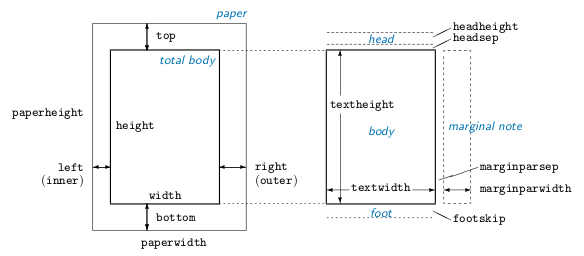
\includegraphics[width=0.8\textwidth]{figures/geometry_margin.png}
  \flushright Fonte: \cite{Umeki:2010:Geometry}
  \caption{Ilustração da opções disponíveis para \lcode{parametro} apresentadas na Tabela \ref{tab:par_geometry}.} \label{fig:par_geometry}
\end{figure}

\subsection{Estilo de página}
Existe um estilo de página definido como padrão\footnote{Corresponde ao estilo
\lcode{plain} apresentado na Tabela \ref{tab:par_style}.}, quando deseja-se
mudar o estilo em todo o documento pode-se utilizar o comando
\begin{code}
  \pagestyle{style}
\end{code}
e quando for necessário mudá-lo apenas na página atual utiliza-se o comando
\begin{code}
  \thispagestyle{style}
\end{code}

As opções para \lcode{style} são apresentadas na Tabela~\ref{tab:par_style}.
\begin{table}[htb]
  \centering
  \caption{Opções disponíveis para \lcode{style}.}
  \label{tab:par_style}
  % File: style@latex-with-vim.tex
% This code is part of LaTeX with Vim.
% 
% Description: LaTeX with Vim is free book about Vim, LaTeX and Git.
% 
% Created: 30.03.12 12:19:38 AM
% Last Change: 30.03.12 12:19:44 AM
% 
% Author: Raniere Gaia Costa da Silva, r.gaia.cs@gmail.com
% Organization:  
% 
% Copyright (c) 2010, 2011, 2012, Raniere Gaia Costa da Silva. All rights 
% reserved.
% 
% This file is license under the terms of a Creative Commons Attribution 
% 3.0 Unported License, or (at your option) any later version. More details
% at <http://creativecommons.org/licenses/by/3.0/>.

\begin{tabular}{lp{0.8\textwidth}}
    \hline
    Código & Descrição \\ \hline
    \lcode{plain} & Imprime os números de página no centro do pé da página. \\
    \lcode{headings} & No cabeçalho de cada página imprime o capítulo que está sendo processado e o número da página. O pé da página fica vazio. \\
    \lcode{empty} & Coloca tanto o cabeçalho como o pé da página vazios.
\end{tabular}

\end{table}

Aos interessados em criar um estilo próprio, sugere-se utilizar o pacote
\lcode{fancyhdr}.

\chapter{Alguns pacotes úteis}
No capítulo anterior foi apresentado três pacotes (\pkgname{inputenc},
\pkgname{babel} e \pkgname{geometry}) que costuma estar presentes em
todo documente LaTeX. Nesse capítulo vamos apresentar alguns outros pacotes mais
alguns pacotes.

\section{Cor}
Para alterar a cor\index{fonte!cor} do texto é necessário os pacotes
\pkgname{graphicx}\index{pacote!graphicx@\pkgname{graphicx}} e
\pkgname{color}\index{pacote!color@\pkgname{color}} e pode-se utilizar um dos
comandos: \lstinline!\textcolor!\index{comando!textcolor@\lstinline+\textcolor+}
ou \lstinline!\color!\index{comando!color@\lstinline+\color+}.

A seguir apresentamos um exemplo. \\
\example{codes/hello_color@latex_with_vim.tex}

\section{Endereços da internet}
Nos endereços da internet é muito comum a presença de caracteres especiais para
o LaTeX. Para inserir um endereço da internet facilmente pode-se utilizar o
comando \lstinline!\verb!\index{comando!verb@\lstinline+\verb+} que foi
apresentado anteriormente ou utilizar o comando
\lstinline!\url!\index{comando!url@\lstinline+\url+} disponível no pacote
\pkgname{url}\index{pacote!url@\pkgname{url}}.

\section{Hiperligação e metadados}
Uma das capacidades do \lcode{pdf} é possuir metadados (informações para serem lidas por
máquinas) e hiperligação internos e/ou externos (marcações ao longo do texto que
possibilita ao usuário uma leitura não linear do documento).

Hiperligações são muito úteis ao leitor para que esse localize facilmente o
texto a que uma referência cruzada refere-se. A criação das hiperligações é
feita ao incluir o pacote \pkgname{hyperref}.

A inclusão de alguns metadados também é feita pelo pacote \pkgname{hyperref}.
Para a inclusão nos metadados do \lcode{pdf} do título e autor da obra pode-se utilizar
\begin{code}
\hypersetup{
  pdfinfo={
    Title={Titulo da obra},
    Author={Nome do autor},
  }
}
\end{code}

\section{Figuras}
No LaTeX é possível inserir figuras\index{figura} contidas em um arquivo de
imagem ou desenhar uma\footnote{Ver a Seção~\ref{sse:tikz}}. Também podemos
adicionar uma legenda para a figura.

\subsection{Arquivos de imagem}
Para inserir arquivos de imagem é necessário o pacote
\pkgname{graphicx}\index{pacote!graphicx@\pkgname{graphicx}}. A imagem a ser
inserida pode encontrar-se em um dos seguintes formatos: \lcode{jpg},
\lcode{png}, \lcode{pdf} ou \lcode{eps}\footnote{Este formato requer instalada o
TeX Live 2011 ou superior pois a partir dessa versão o pacote para conversão do
arquivo \lcode{eps} para um formato suportado é nativa.}.

O comando
\lstinline!\includegraphics!\index{comando!includegraphics@\lstinline+\includegraphics+}
é o responsável por indicar a figura que será inserida, sendo a figura inserida
ao longo do texto. A síntaxe deste comando é
\begin{code}
  \includegraphics[parametro=comprimento]{arquivo}
\end{code}
em que \lcode{parametro} é um comando disponíveis (algumas opções disponíveis
são apresentadas na Tabela \ref{tab:figure_size}), \lcode{comprimento} é uma medida
para \lcode{parametro} e \lcode{arquivo} é o nome do arquivo que contem a imagem.
\begin{table}[!htb]
  \centering
  \caption{Opções disponíveis para \envname{parametro}.}
  \label{tab:figure_size}
  % Filename: figure_size@latex_with_vim.tex
% This code is part of LaTeX with Vim.
% 
% Description: LaTeX with Vim is free book about Vim, LaTeX and Git.
% 
% Created: 30.03.12 12:13:41 AM
% Last Change: 30.03.12 12:13:48 AM
% 
% Author: Raniere Gaia Costa da Silva, r.gaia.cs@gmail.com
% Organization:  
% 
% Copyright (c) 2010, 2011, 2012, Raniere Gaia Costa da Silva. All rights 
% reserved.
% 
% This file is license under the terms of a Creative Commons Attribution 
% 3.0 Unported License, or (at your option) any later version. More details
% at <http://creativecommons.org/licenses/by/3.0/>.
\begin{tabular}{lp{0.8\textwidth}}
    \hline
    Código & Descrição \\ \hline
    \textsf{width} & Corresponde a largura da figura. \\
    \textsf{height} & Corresponde a altura da figura. \\
    \textsf{scale} & Corresponde a escala da figura. \\
    \textsf{angle} & Corresponde a uma rotação no sentido horário. \\
    \textsf{page} & Apenas para \textsf{PDF}'s, indica a página a ser utilizada. \\ \hline
\end{tabular}

\end{table}

Uma dica é que para \lcode{comprimento} podemos utilizar medidas correspondente a
folha escolhida como por exemplo \lstinline!\textwidth! ou
\lstinline!\textheight!.\\
\example{codes/includegraphics@latex_with_vim.tex}

Maiores informações podem ser encontradas em
\url{http://en.wikibooks.org/wiki/LaTeX/Importing_Graphics}.

\subsection{\envname{figure}}
O ambiente \envname{figure}\index{ambiente!figure@\envname{figure}} possibilita
a inclusão de uma legenda para a figura e trabalha a mesma como um objeto
flutuante. A síntaxe deste ambiente é
\begin{code}
  \begin{figure}[place]
    imagem
    \caption{legenda}
    \label{P:imagem}
  \end{figure}
\end{code}
onde \lcode{place} é o parâmetro que indica onde a figura deve ser
preferencialmente inserida (as opções disponíveis são apresentadas na Tabela
\ref{tab:figure_place} e a opção padrão é \lcode{tbp}), \lcode{imagem}
corresponde ao código da figura a ser inserida,
\lstinline!\caption!\index{comando!caption@\lstinline+\caption+} é o comando
correspondente a legenda e \lcode{legenda} é o texto a ser apresentado como
legenda, \lstinline!\label! é o comando para referência cruzada como já
apresentado. \\
\example{codes/figure_centering@latex_with_vim.tex}
\begin{table}[!htb]
  \centering
  \caption{Opções disponíveis para \envname{place}.}
  \label{tab:figure_place}
  % Filename: figure_place@latex_with_vim.tex
% This code is part of LaTeX with Vim.
% 
% Description: LaTeX with Vim is free book about Vim, LaTeX and Git.
% 
% Created: 30.03.12 12:13:22 AM
% Last Change: 30.03.12 12:13:28 AM
% 
% Author: Raniere Gaia Costa da Silva, r.gaia.cs@gmail.com
% Organization:  
% 
% Copyright (c) 2010, 2011, 2012, Raniere Gaia Costa da Silva. All rights 
% reserved.
% 
% This file is license under the terms of a Creative Commons Attribution 
% 3.0 Unported License, or (at your option) any later version. More details
% at <http://creativecommons.org/licenses/by/3.0/>.
\begin{tabular}{lp{0.8\textwidth}}
    \hline
    Código & Descrição \\ \hline
    \textsf{h} & Na posição onde o código se encontra. \\
    \textsf{t} & No topo de uma página. \\
    \textsf{b} & No fim de uma página. \\
    \textsf{p} & Em uma página separada. \\
    \textsf{!} & Modifica algumas configurações a respeito de boa posição para objeto flutuante. \\ \hline
\end{tabular}

\end{table}

Uma dica útil é que o comando
\lstinline!\clearpage!\index{comando!clearpage@\lstinline+\clearpage+} que força
as figuras pendentes a serem inseridas.

Outras informações podem ser encontradas em
\url{http://en.wikibooks.org/wiki/LaTeX/Floats,_Figures_and_Captions}.

% Aula 03 - AMSMATH, TikZ e BibTeX
\chapter{Matemática no \LaTeX, amsmath} \label{sch:math}
Neste capítulo abordaremos o modo matemático do LaTeX, com uma ênfase nos
pacotes amsmath\index{pacote!amsmath@\pkgname{amsmath}}, amsfonts, amssymb e
amsthm.

\section{Modo matemático}
Para que expressões matemáticas seja processadas corretamente, deve-se mudar do
modo texto para o modo matemático, o que pode ser feito de várias maneiras.

A apresentação de expressões matemáticas pode ocorrer de duas maneiras:
\flang{inline}\index{modo matematico@modo matemático!inline@\flang{inline}},
quando aparecem na mesma linha do texto, e \flang{displayed}\index{modo
matematico@modo matemático!displayed@\flang{displayed}}, quando aparecem em uma
linha própria e centralizada (podendo ou não ser numerada\footnote{Deve-se
numerar apenas equações as quais serão feita referências posteriormente.}).

A seguir, informaremos como proceder para produzir expressões matemáticas
\flang{inline} ou \flang{displayed}. Ao final, apresentaremos algumas dicas
sobre o uso de expressões \flang{inline} e \flang{displayed}.

\subsection{\flang{Inline}}
Expressões matemáticas \flang{inline}\index{modo matematico@modo
matemático!inline@\flang{inline}} devem ser iniciadas por \lstinline!$! e
fechadas por \lstinline!$! ou iniciadas por \lstinline!\)! e fechadas por
\lstinline!\)!. \\
\example{codes/math_inline@latex_with_vim.tex}

\subsection{\flang{Displayed}}
Expressões matemáticas \flang{displayed}\index{modo matematico@modo
matemático!displayed@\flang{displayed}} devem ser iniciadas por \lstinline!$$! e
fechadas por \lstinline!$$! ou iniciadas por \lstinline!\[! e fechadas por
\lstinline!\]!. \\
\example{codes/math_display@latex_with_vim.tex}

Alguns ambientes, como \envname{equation}, \envname{eqnarray} e \envname{align},
também produzem expressões matemáticas \flang{displayed}.

\subsection{Uso de \flang{inline} e \flang{displayed}}
Um ótimo resumo sobre quando usar expressões \flang{inline} e \flang{displayed}
encontra-se em
\url{http://www.math.uiuc.edu/~hildebr/tex/displays.html}\nocite{Hildebrand:TeX_Resoures}
e a seguir apresentaremos tradução de alguns trechos. Para maiores detalhes
recomenda-se uma leitura na obra ``Mathematics Into
Type''\nocite{Swanson:1999:Mathematics}.

Expressões \flang{inline} são ``feias'' quando apresentam frações, somatórios,
integrais, \ldots e algumas vezes precisam de um cuidado especial para
respeitarem as margens. Entretanto, deve-se preferir utilizar expressões
\flang{displayed} apenas nas seguintes ocasiões:
\begin{itemize}
  \item a expressão é longa (ocupa mais da metade de uma linha);
  \item a expressão requer bastante espaço vertical, i.e., possui várias
    frações, somatórios, integrais, \ldots;
  \item a equação será numerada;
  \item a expressão que você deseja destacar/enfatizar.
\end{itemize}

\section{Primeiros comandos no modo matemático}
A seguir enunciaremos como proceder para produzir as primeiras equações, mas
antes é importante saber que o modo matemático ignora qualquer espaço (para
inserir um espaço em branco no modo matemático veja a seção
\ref{sss:math:textos_e_espacamentos}).

\subsection{Operações aritméticas básicas}
As operações aritméticas básicas\index{modo matematico@modo matemático!operacoes
aritmeticas basicas@operações aritméticas básicas} são escritas normalmente,
exceto pela multiplicação que utiliza-se dos comandos \lstinline!\times! ou
\lstinline!\cdot!\footnote{O uso do comando mais adequado depende muito do campo
de estudo.} e das frações representada pelo comando
\lstinline!\frac!\footnote{Deve-se ponderar o uso deste comando por questão de
legibilidade.}. \\
\example{codes/math_powers_indices@latex_with_vim.tex}

\subsection{Índices e expoentes}
Índices\index{modo matematico@modo matemático!indice@índice} e
expoentes\index{modo matematico@modo matemático!expoente} são indicados pelos
respectivos comandos: \flang{underscore}, \lcode{_}, e \flang{caret}, \lcode{^}.
Por padrão apenas o primeiro símbolo depois do comando é alterado, quando for
necessário mais de um símbolo deve-se utilizar chaves.

O símbolo \flang{prime}, muito utilizado para derivadas, já vem posicionado
corretamente.\footnote{Algumas vezes deve-se preferir utilizar o comando
\lcode{prime} em conjunto com \flang{underscore} e/ou \flang{caret}.} \\
\example{codes/math_powers_indices@latex_with_vim.tex}

\subsection{Acentos}
Os acentos\index{modo matematico@modo matemático!acento} disponíveis no modo
matemático são apresentados na Tabela~\ref{tab:math_accents}.
\begin{table}[h!tb]
  \centering
  \caption{Acentos disponíveis no modo matemático.}
  \label{tab:math_accents}
  % Filename: math_accents@latex_with_vim.tex
% This code is part of LaTeX with Vim.
% 
% Description: LaTeX with Vim is free book about Vim, LaTeX and Git.
% 
% Created: 30.03.12 12:14:55 AM
% Last Change: 30.03.12 12:15:01 AM
% 
% Author: Raniere Gaia Costa da Silva, r.gaia.cs@gmail.com
% Organization:  
% 
% Copyright (c) 2010, 2011, 2012, Raniere Gaia Costa da Silva. All rights 
% reserved.
% 
% This file is license under the terms of a Creative Commons Attribution 
% 3.0 Unported License, or (at your option) any later version. More details
% at <http://creativecommons.org/licenses/by/3.0/>.
\begin{tabular}{cc|cc|cc}
    \hline
    Comando & Resultado & Comando & Resultado & Comando & Resultado \\ \hline
    \textbackslash\textsf{acute\{a\}} & $\acute{a}$ & \textbackslash\textsf{bar\{a\}} & $\bar{a}$ & \textbackslash\textsf{breve\{a\}} & $\breve{a}$ \\
    \textbackslash\textsf{check\{a\}} & $\check{a}$ & \textbackslash\textsf{dot\{a\}} & $\dot{a}$ & \textbackslash\textsf{ddot\{a\}} & $\ddot{a}$ \\
    \textbackslash\textsf{dddot\{a\}} & $\dddot{a}$ & \textbackslash\textsf{ddddot\{a\}} & $\ddddot{a}$ & \textbackslash\textsf{grave\{a\}} & $\grave{a}$ \\
    \textbackslash\textsf{hat\{a\}} & $\hat{a}$ & \textbackslash\textsf{widehat\{a\}} & $\widehat{a}$ & \textbackslash\textsf{mathring\{a\}} & $\mathring{a}$ \\
    \textbackslash\textsf{tilde\{a\}} & $\tilde{a}$ & \textbackslash\textsf{widetilde\{a\}} & $\widetilde{a}$ & \textbackslash\textsf{vec\{a\}} & $\vec{a}$ \hfill
\end{tabular}

\end{table}

\subsection{Delimitadores}
Parênteses\index{modo matematico@modo
matemático!parenteses@parênteses|see{delimitadores}}, colchetes\index{modo
matematico@modo matemático!colchetes|see{delimitadores}} e chaves\index{modo
matematico@modo matemático!chaves|see{delimitadores}} são exemplos de
delimitadores\index{modo matematico@modo matemático!delimitadores}. Uma lista
completa dos delimitadores disponíveis no LaTeX encontra-se na
Tabela~\ref{tab:math_delimiter}.
\begin{table}[h!tb]
  \centering
  \caption{Delimitadores disponíveis no LaTeX.}
  \label{tab:math_delimiter}
  % Filename: math_delimiter@latex_with_vim.tex
% This code is part of LaTeX with Vim.
% 
% Description: LaTeX with Vim is free book about Vim, LaTeX and Git.
% 
% Created: 30.03.12 12:16:24 AM
% Last Change: 30.03.12 12:16:29 AM
% 
% Author: Raniere Gaia Costa da Silva, r.gaia.cs@gmail.com
% Organization:  
% 
% Copyright (c) 2010, 2011, 2012, Raniere Gaia Costa da Silva. All rights 
% reserved.
% 
% This file is license under the terms of a Creative Commons Attribution 
% 3.0 Unported License, or (at your option) any later version. More details
% at <http://creativecommons.org/licenses/by/3.0/>.
\begin{tabular}{>{\centering}p{0.13\linewidth}<{\centering}>{\centering}p{0.07\linewidth}<{\centering}|>{\centering}p{0.13\linewidth}<{\centering}>{\centering}p{0.07\linewidth}<{\centering}|>{\centering}p{0.13\linewidth}<{\centering}>{\centering}p{0.07\linewidth}<{\centering}|>{\centering}p{0.13\linewidth}<{\centering}>{\centering}p{0.07\linewidth}<{\centering}}
    \hline
    Com. & Res. & Com. & Res. & Com. & Res. & Com. & Res. \tabularnewline \hline
    \lstinline!(! & $($ & \lstinline!)! & $)$ & \lstinline![! & $[$ & \lstinline!]! & $]$ \tabularnewline
    \lstinline!\{! & $\{$ & \lstinline!\}! & $\}$ & \lstinline!\backslash! & $\backslash$ & \lstinline!/! & $/$ \tabularnewline
    \lstinline!\langle! & $\langle$ & \lstinline!\rangle! & $\rangle$ & \lstinline!|! & $|$ & \lstinline!\|! & $\|$ \tabularnewline
    \lstinline!\lfloor! & $\lfloor$ & \lstinline!\rfloor! & $\rfloor$ & \lstinline!\lceil! & $\lceil$ & \lstinline!\rceil! & $\rceil$ \tabularnewline
    \lstinline!\ulcorner! & $\ulcorner$ & \lstinline!\urcorner! & $\urcorner$ &\lstinline!\llcorner! & $\llcorner$ & \lstinline!\lrcorner! & $\lrcorner$ \tabularnewline \hline
\end{tabular}
\begin{flushleft}
    \textbf{Nota:} Enquanto que \lstinline!|! \'{e} um limitador \lstinline!\mid! \'{e} um operador l\'{o}gico.
\end{flushleft}

\end{table}

Para expressões matemáticas no modo \flang{displayed} ou longas é aconselhável
utilizar os comandos \lstinline!\left! e \lstinline!\right! anteriormente ao
limitador para ajustá-lo verticalmente. \\
\example{codes/math_delimiters_sizes@latex_with_vim.tex}

\subsection{Textos e espaçamentos} \label{sss:math:textos_e_espacamentos}
Existem três ocasiões em que é preciso inserir um texto\index{modo
matematico@modo matemático!texto} dentro de uma expressão matemática:
\begin{itemize}
  \item um operador matemático é representado pelas primeiras letras de seu nome, e.g., $\max$, $\min$, $\lim$, \ldots;
  \item uma variável é representada por mais de uma letra;
  \item incluir uma explicação/justificativa.
\end{itemize}

O LaTeX já possui vários operadores matemáticos definidos (são apresentados mais
a frente) e quando o operador desejado não estiver definido deve-se utilizar o
comando \lstinline!\operatorname!\index{modo matematico@modo matemático!novos
operadores} ou \lstinline!\DeclareMathOperator!, este último quando o operador
for ser utilizado várias vezes no documento. 

Em relação ao nome de variáveis\index{modo matematico@modo matemático!nomes
longos para variaveis@nomes longos para variáveis}, deve-se evitar ao máximo
nomeá-las com mais de uma letra (utilizar o alfabeto grego para isso). Quando
não for possível evitar, deve-se utilizar o comando \lstinline!\mathrm! para
evitar confusões. \\
\example{codes/math_var_names@latex_with_vim.tex}

Já para a inclusão de textos explicativos deve-se utilizar o comando
\lstinline!\text!\index{comando!text@\lstinline+\text+} e
\lstinline!\intertext!, este último reservado apenas para expressões
\flang{displayed}. \\
\example{codes/math_text@latex_with_vim.tex}

Quanto ao espaçamento\index{modo matematico@modo
matemático!espacamento@espaçamento}, normalmente não é preciso se preocupar com
este pois o LaTeX inclui o espaçamento adequado. Em raras ocasiões deve-se
incluir algum espaço apresentado na Tabela~\ref{tab:math_spacing}.
\begin{table}[!htb]
  \centering
  \caption{Espaçamento no modo matemático.}
  % Filename: algorithmic@latex_with_vim.tex
% This code is part of LaTeX with Vim.
% 
% Description: LaTeX with Vim is free book about Vim, LaTeX and Git.
% 
% Created: 30.03.12 12:11:31 AM
% Last Change: 30.03.12 12:11:38 AM
% 
% Author: Raniere Gaia Costa da Silva, r.gaia.cs@gmail.com
% Organization:  
% 
% Copyright (c) 2010, 2011, 2012, Raniere Gaia Costa da Silva. All rights 
% reserved.
% 
% This file is license under the terms of a Creative Commons Attribution 
% 3.0 Unported License, or (at your option) any later version. More details
% at <http://creativecommons.org/licenses/by/3.0/>.
\begin{tabular}{>{\centering}p{0.1\linewidth}<{\centering}>{\centering}p{0.15\linewidth}<{\centering}>{\centering}p{0.15\linewidth}<{\centering}|>{\centering}p{0.1\linewidth}<{\centering}>{\centering}p{0.15\linewidth}<{\centering}>{\centering}p{0.15\linewidth}<{\centering}}
    \hline
    Abrev. & Comando & Exemplo & Abrev. & Comando & Exemplo \tabularnewline \hline
    & sem espa\c{c}o & $\Rightarrow \Leftarrow$ & \lstinline!\,! & \lstinline!\thinspace! & $\Rightarrow \, \Leftarrow$ \tabularnewline
    \lstinline!\:! & \lstinline!\medspace! & $\Rightarrow \; \Leftarrow$ & \lstinline!\;! & \lstinline!\thickspace! & $\Rightarrow \; \Leftarrow$ \tabularnewline
    & \lstinline!\quad! & $\Rightarrow \quad \Leftarrow$ & & \lstinline!\qquad! & $\Rightarrow \qquad \Leftarrow$ \tabularnewline \hline
\end{tabular}

  \label{tab:math_spacing}
\end{table}
Uma dessas ocasiões é em integrais. \\
\example{codes/math_space_integral@latex_with_vim.tex}

\subsection{Matrizes}
Para a construção de matrizes\index{modo matematico@modo matemático!matrizes} (e
vetores\index{modo matematico@modo matemático!vetores|see{matrizes}}) utiliza-se
o ambiente \envname{matrix} onde as colunas são separadas por \lstinline!&! e as
linhas por \lstinline!\\!. \\
\example{codes/math_matrix@latex_with_vim.tex}

Destaca-se que o ambiente \envname{matrix} só pode ser utilizado dentro do
ambiente matemático e que na última linha não utiliza-se o comando
\lstinline!\\!\index{comando! @\lstinline+\\+}.

Pode-se utilizar limitadores envolvendo o ambiente \envname{matrix} ou utilizar
uma variante: \envname{pmatrix}, \envname{bmatrix}, \envname{Bmatrix},
\envname{vmatrix} ou \envname{Vmatrix} que corresponde, respectivamente, aos
delimitadores $( )$, $[ ]$, $\{ \}$, $| |$ e $\| \|$. \\

\section{Comandos avançados no modo matemático}
\subsection{Equações, numeração e referenciação} \label{sse:latex:equation}
Para o uso de expressões matemáticas a serem referenciadas\index{modo
matematico@modo matemático!numeracao@numeração} posteriormente, recomenda-se o
ambiente \envname{equation}\index{ambiente!equation@\envname{equation}} em
conjunto com o comando
\lstinline!\label!\index{comando!label@\lstinline+\label+}. \\
\example{codes/math_equation@latex_with_vim.tex}

No exemplo acima, \lcode{E:TeoPit} correspondente ao parâmetro do comando
\lstinline!\label!, como apresentado na Seção~\ref{sse:cross_reference}. A
referência a equação ocorre pelo comando \lstinline!\eqref!. \\
\example{codes/math_equation_eqref@latex_with_vim.tex}

\subsection{\flang{Tags}}
O comando \lstinline!\tag!\index{comando!tag@\lstinline+\tag+} do LaTeX nomeia
uma equação\index{modo matematico@modo matemático!tag@\flang{tag}} e a
referência passa a ser feito por este. \\
\example{codes/math_equation_tag@latex_with_vim.tex}

Vale destacar que podemos utilizar o comando \lstinline!\label! como parâmetro
do comando \lstinline!\tag!.

\subsection{Teorema}
O comando \lstinline{\newtheorem}\index{modo matematico@modo matemático!teorema}
deve ser inserido no \textit{preâmbulo} e é responsável por criar um ambiente
numerado para informações. Sua sintaxe é
\begin{code}
  \newtheorem{nome}{texto}
\end{code}
onde \lcode{nome} é o nome do ambiente a ser criado e \lcode{texto} é a
sequência de caracteres que precede a numeração. Caso deseje-se não numerar
deve-se utilizar a sintaxe
\begin{code}
  \newtheorem*{nome}{texto}
\end{code}

Para fazer uso do novo ambiente deve-se utilizar a sintaxe padrão para um
ambiente
\begin{code}
  \begin{nome}
    ...
  \end{nome}
\end{code}
ou ainda
\begin{code}
  \begin{nome}[XXX]
    ...
  \end{nome}
\end{code}
onde \lcode{XXX} é uma sequência de caracteres que aparece entre parênteses logo
após a numeração.

\subsection{Demonstração}
O ambiente \envname{proof} é destinada a demonstrações\index{modo
matematico@modo matemático!demonstracao@demonstração} e caracterizado por
terminar com o comando \lstinline!\qed!. \\
\example{codes/math_proof@latex_with_vim.tex}

O ambiente \envname{proof}, como podemos observar no exemplo abaixo, não
trabalha adequadamente quando é finalizado com uma expressão matemática
\flang{displayed} e para corrigir isso devemos informar onde onde será inserido
o símbolo \flang{qed}. \\
\example{codes/math_proof_set_qed@latex_with_vim.tex}

\subsection{Alinhamento}
O ambiente \envname{equation} foi projetado para trabalhar apenas com equações
de uma única linha, nesta seção vamos apresentar algumas formas de trabalhar com
equações com várias linhas\index{modo matematico@modo matemático!multiplas
equacoes@múltiplas equações}.

Para múltiplas equações alinhadas utilizamos o ambiente
\envname{align}\index{ambiente!align@\envname{align}}, sendo cada linha separada
pelo comando \lstinline!\\!\index{comando! @\lstinline+\\+} e o alinhamento por
\lstinline!&!\index{comando! @\lstinline+&+}. \\
\example{codes/math_align@latex_with_vim.tex}

Quando o alinhamento ocorrer adjacente a um sinal de \lstinline!=!,
\lstinline!+!, \dots devemos utilizar o comando \lstinline!&! antes do sinal.

O ambiente \envname{align} numera todas as equações. Caso não queira numerar uma
ou mais equações deve-se utilizar o comando \lstinline!\notag! em cada linha
correspondente.

O comando \lstinline!\label! deve estar presente em cada linha.

Quando desejar adicionar a alguma linha alguma anotação utiliza-se o comando
\lstinline!&&! entre a equação e a anotação. \\
\example{codes/math_align_annotation@latex_with_vim.tex}

\subsection{Fórmulas longas}
Fórmulas muito longas é fonte de vários problemas ao utilizar o LaTeX. Se
existir fórmulas muito longas na obra que estiver trabalhando sugere-se inserir
o pacote \pkgname{breqn} por este quebrá-las automaticamente ao utilizar o
ambiente \envname{dmath} no lugar de \envname{equation}.

Infelizmente o pacote \pkgname{breqn} nem sempre funciona como desejado e nesses
casos a solução é fazer a quebra da equação manualmente. Para isso, deve-se
utilizar o ambiente \envname{multline}, para uma única equação, ou
\envname{split}, este último deve ser utilizado dentro de um outro ambiente
matemático. Se for quebrar as equações manualmente, recomenda-se ler a seção
``Split equations without alignment'' de ``User’s Guide for the amsmath Package''.

\subsection{Ocultando termos}
Ao trabalhar com fórmulas muito longas tenta-se diminuir o tamanho utilizando
sequências e muitas vezes é aconselhável indicar o número de termos. Para isso
podemos utilizar os comandos \lstinline!\overbrace! ou \lstinline!\underbrace!.
\\
\example{codes/math_underbrace@latex_with_vim.tex}

\subsection{Funções definidas por partes}
É relativamente comum definirmos uma equações por partes e o ambiente adequado
para representar esta construção é o \envname{cases}\index{modo matematico@modo
matemático!funcoes definidas por partes@funções definidas por partes}. \\
\example{codes/math_cases@latex_with_vim.tex}

O ambiente \envname{cases}\index{modo matematico@modo matemático!sistemas de
equacoes@sistemas de equações} também pode ser utilizado para sistemas de
equações.

\subsection{Fonte e Símbolos}
No modo matemático, o LaTeX classifica os caracteres em alfabeto matemático e
símbolos matemáticos. Baseado nessa classificação escolhe uma fonte a ser usada.

Para alterar a fonte de caracteres do alfabeto matemático utiliza-se o comando
\lstinline!\mathXX! sendo que \lcode{XX} corresponde ao código da fonte a ser
utilizada. A Tabela~\ref{tab:op_amfonte} apresenta alguns das opções
disponíveis.
\begin{table}[h!tb]
  \centering
  \caption{Opções disponíveis para \lcode{XX} da fonte para o alfabeto matemático.}
  \label{tab:op_amfonte}
  % Filename: math_op_amfonte@latex_with_vim.tex
% This code is part of LaTeX with Vim.
% 
% Description: LaTeX with Vim is free book about Vim, LaTeX and Git.
% 
% Created: 30.03.12 12:11:31 AM
% Last Change: 30.03.12 12:11:38 AM
% 
% Author: Raniere Gaia Costa da Silva, r.gaia.cs@gmail.com
% Organization:  
% 
% Copyright (c) 2010, 2011, 2012, Raniere Gaia Costa da Silva. All rights 
% reserved.
% 
% This file is license under the terms of a Creative Commons Attribution 
% 3.0 Unported License, or (at your option) any later version. More details
% at <http://creativecommons.org/licenses/by/3.0/>.
\begin{tabular}{lp{0.8\textwidth}}
    \hline
    Código & Descrição \\ \hline
    \lcode{it} & Texto em itálico. \\
    \lcode{bf} & Texto em negrito. \\
    \lcode{rm} & Texto em romano. \\
    \lcode{sf} & Texto em sans serif. \\
    \lcode{tt} & Texto na tipografia de uma máquina de escrever.
\end{tabular}

\end{table}

A seguir é ilustrado as opções apresentadas na Tabela \ref{tab:op_amfonte}. \\
\example{codes/math_op_amfonte@latex_with_vim.tex}

Para símbolos matemáticos apenas é possível apresentá-los em negrito e, para
isso, utiliza-se o comando \lstinline!\boldsymbol!. \\
\example{codes/math_boldsymbol@latex_with_vim.tex}

No LaTeX também existe quatro alfabetos que são interpretados como símbolos. Um
deles é o alfabeto grego, apresentado no capítulo anterior e os outros três são
acessados com o comando \lstinline!\mathXX!, sendo que \lcode{XX} corresponde ao
código da fonte a ser utilizada. A Tabela~\ref{tab:op_asfonte} apresenta as
opções disponíveis.
\begin{table}[h!tb]
  \centering
  \caption{Opções disponíveis para \lcode{XX} da fonte para o alfabeto matemático interpretado como símbolo.}
  \label{tab:op_asfonte}
  % Filename: math_op_asfonte@latex_with_vim.tex
% This code is part of 'LaTeX with Vim'.
% 
% Description: This file correspond to a example of LaTeX producing newlines.
% 
% Created: 27.06.12 08:29:06 AM
% Last Change: 27.06.12 08:29:06 AM
% 
% Author: Raniere Gaia Costa da Silva, r.gaia.cs@gmail.com
% 
% Copyright (c) 2012, Raniere Gaia Costa da Silva. All rights 
% reserved.
% 
% This work is licensed under the Creative Commons Attribution-ShareAlike 3.0 Unported License. To view a copy of this license, visit http://creativecommons.org/licenses/by-sa/3.0/ or send a letter to Creative Commons, 444 Castro Street, Suite 900, Mountain View, California, 94041, USA.
%
\begin{tabular}{lp{0.8\textwidth}}
    \hline
    Código & Descrição \\ \hline
    \lcode{cal} & Texto em caligráfico, apenas para caixa alta. \\
    \lcode{frak} & Texto em Euler Fraktur. \\
    \lcode{bb} & Texto em blackboard bold, apenas para caixa alta.
\end{tabular}

\end{table}

A seguir é ilustrado as opções apresentadas na Tabela~\ref{tab:op_asfonte}. \\
\example{codes/math_op_asfonte@latex_with_vim.tex}

Destaca-se que a fonte blackboard bold é normalmente utilizada para representar
os conjuntos dos números naturais ($\mathbb{N}$), inteiros ($\mathbb{Z}$), reais
($\mathbb{R}$) e complexos ($\mathbb{C}$).

\section{Símbolos e operadores}
A seguir apresentaremos vários dos símbolos e operadores disponíveis no LaTeX.
Para uma lista completa recomenda-se ``The Comprehensive LaTeX Symbol
List''\nocite{Pakin:2009:Symbol}. Ao final, abordamos os comandos para raiz
quadrada, binomial e congruências.
\begin{table}[h!tb]
  \centering
  \caption{Setas}
  \label{tab:math_arrows}
  % Filename: math_arrows@latex_with_vim.tex
% This code is part of LaTeX with Vim.
% 
% Description: LaTeX with Vim is free book about Vim, LaTeX and Git.
% 
% Created: 30.03.12 12:15:12 AM
% Last Change: 30.03.12 12:15:22 AM
% 
% Author: Raniere Gaia Costa da Silva, r.gaia.cs@gmail.com
% Organization:  
% 
% Copyright (c) 2010, 2011, 2012, Raniere Gaia Costa da Silva. All rights 
% reserved.
% 
% This file is license under the terms of a Creative Commons Attribution 
% 3.0 Unported License, or (at your option) any later version. More details
% at <http://creativecommons.org/licenses/by/3.0/>.
\begin{tabular}{cc|cc|cc}
    \hline
    Com. & Res. & Com. & Res. & Com. & Res. \\ \hline
    \lstinline!\leftarrow! & $\leftarrow$ & \lstinline!\rightarrow! & $\rightarrow$ & \lstinline!\longleftarrow! & $\longleftarrow$ \\
    \lstinline!\longrightarrow! & $\longrightarrow$ & \lstinline!\Leftarrow! & $\Leftarrow$ & \lstinline!\Rightarrow! & $\Rightarrow$ \\
    \lstinline!\Longleftarrow! & $\Longleftarrow$ & \lstinline!\Longrightarrow! & $\Longrightarrow$ & \lstinline!\nleftarrow! & $\nleftarrow$ \\
    \lstinline!\nrightarrow! & $\nrightarrow$ & \lstinline!\nLeftarrow! & $\nLeftarrow$ & \lstinline!\nRightarrow! & $\nRightarrow$ \\
    \lstinline!\leftrightarrow! & $\leftrightarrow$ & \lstinline!\longleftrightarrow! & $\longleftrightarrow$ & \lstinline!\Leftrightarrow! & $\Leftrightarrow$ \\
    \lstinline!\Longleftrightarrow! & $\Longleftrightarrow$ & \lstinline!\nleftrightarrow! & $\nleftrightarrow$ & \lstinline!\nLeftrightarrow! & $\nLeftrightarrow$ \\
    \lstinline!\dashleftarrow! & $\dashleftarrow$ & \lstinline!\dashrightarrow! & $\dashrightarrow$ & \lstinline!\leftrightharpoons! & $\leftrightharpoons$ \\
    \lstinline!\rightleftharpoons! & $\rightleftharpoons$ & \lstinline!\leftrightarrows! & $\leftrightarrows$ & \lstinline!\rightleftarrows! & $\rightleftarrows$ \\
    \lstinline!\mapsto! & $\mapsto$ & \lstinline!\longmapsto! & $\longmapsto$ & \lstinline!\iff! & $\iff$ \\
    \lstinline!\uparrow! & $\uparrow$ & \lstinline!\downarrow! & $\downarrow$ & \lstinline!\Uparrow! & $\Uparrow$ \\
    \lstinline!\Downarrow! & $\Downarrow$ & \lstinline!\updownarrow! & $\updownarrow$ & \lstinline!\Updownarrow! & $\Updownarrow$ \\
    \lstinline!\Lsh! & $\Lsh$ & \lstinline!\Rsh! & $\Rsh$ & \lstinline!\curvearrowleft! & $\curvearrowleft$ \\
    \lstinline!\curvearrowright! & $\curvearrowright$ & \lstinline!\circlearrowleft! & $\circlearrowleft$ & \lstinline!\circlearrowright! & $\circlearrowright$ \\ \hline
\end{tabular}

\end{table}
\begin{table}[!htbp]
  \caption{Relações binárias} \centering
  \label{tab:math_binary_relations}
  % Filename: math_binary_relations@latex_with_vim.tex
% This code is part of LaTeX with Vim.
% 
% Description: LaTeX with Vim is free book about Vim, LaTeX and Git.
% 
% Created: 30.03.12 12:15:58 AM
% Last Change: 30.03.12 12:16:09 AM
% 
% Author: Raniere Gaia Costa da Silva, r.gaia.cs@gmail.com
% Organization:  
% 
% Copyright (c) 2010, 2011, 2012, Raniere Gaia Costa da Silva. All rights 
% reserved.
% 
% This file is license under the terms of a Creative Commons Attribution 
% 3.0 Unported License, or (at your option) any later version. More details
% at <http://creativecommons.org/licenses/by/3.0/>.
\begin{tabular}{cc|cc|cc}
    \hline
    Com. & Res. & Com. & Res. & Com. & Res. \\ \hline
    \lstinline!<! & $<$ & \lstinline!\nless! & $\nless$ & \lstinline!>! & $>$ \\
    \lstinline!\ngtr! & $\ngtr$ & \lstinline!\ll! & $\ll$ & \lstinline!\lll! & $\lll$ \\
    \lstinline!\gg! & $\gg$ & \lstinline!\ggg! & $\ggg$ & \lstinline!=! & $=$ \\
    \lstinline!\neq! & $\neq$ & \lstinline!:! & $:$ & \lstinline!\doteq! & $\doteq$ \\
    \lstinline!\sim! & $\sim$ & \lstinline!\nsim! & $\nsim$ & \lstinline!\cong! & $\cong$ \\
    \lstinline!\ncong! & $\ncong$ & \lstinline!\simeq! & $\simeq$ & \lstinline!\approx! & $\approx$ \\
    \lstinline!\equiv! & $\equiv$ & \lstinline!\leq! ou \lstinline!\le! & $\leq$ & \lstinline!\nleq! & $\nleq$ \\
    \lstinline!\geq! ou \lstinline!\ge! & $\geq$ & \lstinline!\ngeq! & $\ngeq$ & \lstinline!\leqslant! & $\leqslant$ \\
    \lstinline!\nleqslant! & $\nleqslant$ & \lstinline!\geqslant! & $\geqslant$ & \lstinline!\ngeqslant! & $\ngeqslant$ \\
    \lstinline!\eqslantless! & $\eqslantless$ & \lstinline!\eqslantgtr! & $\eqslantgtr$ & \lstinline!\leqq! & $\leqq$ \\
    \lstinline!\nleqq! & $\nleqq$ & \lstinline!\geqq! & $\geqq$ & \lstinline!\ngeqq! & $\ngeqq$ \\
    \lstinline!\lesssim! & $\lesssim$ & \lstinline!\lessapprox! & $\lessapprox$ & \lstinline!\gtrsim! & $\gtrsim$ \\
    \lstinline!\gtrapprox! & $\gtrapprox$ & \lstinline!\prec! & $\prec$ & \lstinline!\nprec! & $\nprec$ \\
    \lstinline!\succ! & $\succ$ & \lstinline!\nsucc! & $\nsucc$ & \lstinline!\preceq! & $\preceq$ \\
    \lstinline!\npreceq! & $\npreceq$  & \lstinline!\succeq! & $\succeq$ & \lstinline!\nsucceq! & $\nsucceq$ \\
    \lstinline!\in! & $\in$ & \lstinline!\notin! & $\notin$ & \lstinline!\owns! & $\owns$ \\
    \lstinline!\subset! & $\subset$ & \lstinline!\supset! & $\supset$ & \lstinline!\subseteq! & $\subseteq$ \\
    \lstinline!\nsubseteq! & $\nsubseteq$ & \lstinline!\supseteq! & $\supseteq$ & \lstinline!\nsupseteq! & $\nsupseteq$ \\
    \lstinline!\subseteqq! & $\subseteqq$ & \lstinline!\nsubseteqq! & $\nsubseteqq$ & \lstinline!\supseteqq! & $\supseteqq$ \\
    \lstinline!\nsupseteqq! & $\nsupseteqq$ & \lstinline!\sqsubset! & $\sqsubset$ & \lstinline!\sqsubseteq! & $\sqsubseteq$ \\
    \lstinline!\sqsupset! & $\sqsupset$ & \lstinline!\sqsupseteq! & $\sqsupseteq$ & \lstinline!\smile! & $\smile$ \\
    \lstinline!\smallsmile! & $\smallsmile$ & \lstinline!\frown! & $\frown$ & \lstinline!\smallfrown! & $\smallfrown$ \\
    \lstinline!\perp! & $\perp$ & \lstinline!\models! & $\models$ & \lstinline!\mid! & $\mid$ \\
    \lstinline!\nmid! & $\nmid$ & \lstinline!\parallel! & $\parallel$ & \lstinline!\nparallel! & $\nparallel$ \\
    \lstinline!\shortmid! & $\shortmid$ & \lstinline!\nshortmid! & $\nshortmid$ & \lstinline!\shortparallel! & $\shortparallel$ \\
    \lstinline!\nshortparallel! & $\nshortparallel$ & \lstinline!\vdash! & $\vdash$ & \lstinline!\nvdash! & $\nvdash$ \\
    \lstinline!\dashv! & $\dashv$ & \lstinline!\vDash! & $\vDash$ & \lstinline!\nvDash! & $\nvDash$ \\
    \lstinline!\Vdash! & $\Vdash $ & \lstinline!\nVdash! & $\nVdash$ & \lstinline!\propto! & $\propto$ \\
    \lstinline!\asymp! & $\asymp$ & \lstinline!\bowtie! & $\bowtie$ & \lstinline!\Join! & $\Join$ \\
    \lstinline!\vartriangleleft! & $\vartriangleleft$ & \lstinline!\ntriangleleft! & $\ntriangleleft$ & \lstinline!\vartriangleright! & $\vartriangleright$ \\
    \lstinline!\ntriangleright! & $\ntriangleright$ & \lstinline!\trianglelefteq! & $\trianglelefteq$ & \lstinline!\ntrianglelefteq! & $\ntrianglelefteq$ \\
    \lstinline!\trianglerighteq! & $\trianglerighteq$ & \lstinline!\ntrianglerighteq! & $\ntrianglerighteq$ &  \lstinline!\blacktriangleleft! & $\blacktriangleleft$ \\
    \lstinline!\blacktriangleright! & $\blacktriangleright$ & \lstinline!\between! & $\between$ & \lstinline!\pitchfork! & $\pitchfork$ \\
    \lstinline!\therefore! & $\therefore$ & \lstinline!\because! & $\because$ \\ \hline
\end{tabular}
\begin{flushleft}
    Enquanto que \lstinline!|! \'{e} um limitador, \lstinline!\mid! \'{e} um operador que corresponde a express\~{a}o ``tal que''.
\end{flushleft}

\end{table}
\begin{table}[!htb]
  \centering
  \caption{Operadores binários}
  \label{tab:math_binary_operations}
  % Filename: math_binary_operations@latex_with_vim.tex
% This code is part of LaTeX with Vim.
% 
% Description: LaTeX with Vim is free book about Vim, LaTeX and Git.
% 
% Created: 30.03.12 12:15:37 AM
% Last Change: 30.03.12 12:15:42 AM
% 
% Author: Raniere Gaia Costa da Silva, r.gaia.cs@gmail.com
% Organization:  
% 
% Copyright (c) 2010, 2011, 2012, Raniere Gaia Costa da Silva. All rights 
% reserved.
% 
% This file is license under the terms of a Creative Commons Attribution 
% 3.0 Unported License, or (at your option) any later version. More details
% at <http://creativecommons.org/licenses/by/3.0/>.
\begin{tabular}{cc|cc|cc}
    \hline
    Com. & Res. & Com. & Res. & Com. & Res. \\ \hline
    \lstinline!+! & $+$ & \lstinline!-! & $-$ & \lstinline!\pm! & $\pm$ \\
    \lstinline!\mp! & $\mp$ & \lstinline!\times! & $\times$ & \lstinline!\cdot! & $\cdot$ \\
    \lstinline!\div! & $\div$ & \lstinline!\And! & $\And$ & \lstinline!\setminus! & $\setminus$ \\
    \lstinline!\smallsetminus! & $\smallsetminus$ & \lstinline!\dagger! & $\dagger$ & \lstinline!\ddagger! & $\ddagger$ \\
    \lstinline!\ast! & $\ast$ & \lstinline!\star! & $\star$ & \lstinline!\wedge! & $\wedge$ \\
    \lstinline!\vee! & $\vee$ & \lstinline!\cap! & $\cap$ & \lstinline!\cup! & $\cup$ \\
    \lstinline!\sqcap! & $\sqcap$ & \lstinline!\sqcup! & $\sqcup$ & \lstinline!\oplus! & $\oplus$ \\
    \lstinline!\ominus! & $\ominus$ & \lstinline!\otimes! & $\otimes$ & \lstinline!\oslash! & $\oslash$ \\
    \lstinline!\odot! & $\odot$ & \lstinline!\bigcirc! & $\bigcirc$ & \lstinline!\circ! & $\circ$ \\
    \lstinline!\bullet! & $\bullet$ & \lstinline!\bigtriangleup! & $\bigtriangleup$ & \lstinline!\bigtriangledown! & $\bigtriangledown$ \\
    \lstinline!\triangleleft! & $\triangleleft$ & \lstinline!\triangleright! & $\triangleright$ &\lstinline!\diamond! & $\diamond$ \\
    \lstinline!\wr! & $\wr$ & \lstinline!\amalg! & $\amalg$ \\ \hline
\end{tabular}

\end{table}
\begin{table}[!htb]
  \centering
  \caption{Operadores puros.}
  \label{tab:math_functions1}
  % Filename: math_functions1@latex_with_vim.tex
% This code is part of LaTeX with Vim.
% 
% Description: LaTeX with Vim is free book about Vim, LaTeX and Git.
% 
% Created: 30.03.12 12:16:46 AM
% Last Change: 30.03.12 12:16:51 AM
% 
% Author: Raniere Gaia Costa da Silva, r.gaia.cs@gmail.com
% Organization:  
% 
% Copyright (c) 2010, 2011, 2012, Raniere Gaia Costa da Silva. All rights 
% reserved.
% 
% This file is license under the terms of a Creative Commons Attribution 
% 3.0 Unported License, or (at your option) any later version. More details
% at <http://creativecommons.org/licenses/by/3.0/>.
\begin{tabular}{cc|cc|cc}
    \hline
    Com. & Res. & Com. & Res. & Com. & Res. \\ \hline
    \lstinline!\log! & $\log$ & \lstinline!\ln! & $\ln$ & \lstinline!\exp! & $\exp$ \\
    \lstinline!\arccos! & $\arccos$ & \lstinline!\arcsin! & $\arcsin$ & \lstinline!\arctan! & $\arctan$ \\
    \lstinline!\cos! & $\cos$ & \lstinline!\sin! & $\sin$ & \lstinline!\tan! & $\tan$ \\
    \lstinline!\csc! & $\csc$ & \lstinline!\sec! & $\sec$ & \lstinline!\cot! & $\cot$ \\
    \lstinline!\cosh! & $\cosh$ & \lstinline!\sinh! & $\sinh$ & \lstinline!\tanh! & $\tanh$ \\
    \lstinline!\lg! & $\lg$ & \lstinline!\arg! & $\arg$ & \lstinline!\hom! & $\hom$ \\
    \lstinline!\dim! & $\dim$ & \lstinline!\ker! & $\ker$ & \lstinline!\det! & $\det$ \\
    \lstinline!\gcd! & $\gcd$ & & & & \\ \hline
\end{tabular}

\end{table}
\begin{table}[!htb]
  \centering
  \caption{Operadores com intervalos.}
  \label{tab:math_functions2}
  % Filename: math_functions2@latex_with_vim.tex
% This code is part of LaTeX with Vim.
% 
% Description: LaTeX with Vim is free book about Vim, LaTeX and Git.
% 
% Created: 30.03.12 12:17:02 AM
% Last Change: 30.03.12 12:17:06 AM
% 
% Author: Raniere Gaia Costa da Silva, r.gaia.cs@gmail.com
% Organization:  
% 
% Copyright (c) 2010, 2011, 2012, Raniere Gaia Costa da Silva. All rights 
% reserved.
% 
% This file is license under the terms of a Creative Commons Attribution 
% 3.0 Unported License, or (at your option) any later version. More details
% at <http://creativecommons.org/licenses/by/3.0/>.
\begin{tabular}{cc|cc|cc|cc}
    \hline
    Comando & Resultado & Comando & Resultado & Comando & Resultado & Comando & Resultado \\ \hline
    \textbackslash\textsf{int} & $\int$ & \textbackslash\textsf{iint} & $\iint$ & \textbackslash\textsf{iiint} & $\iiint$ & \textbackslash\textsf{iiiint} & $\iiiint$ \\
    \textbackslash\textsf{idotsint} & $\idotsint$ & \textbackslash\textsf{oint} & $\oint$ & \textbackslash\textsf{prod} & $\prod$ & \textbackslash\textsf{coprod} & $\coprod$ \\ 
    \textbackslash\textsf{bigcap} & $\bigcap$ & \textbackslash\textsf{bigcup} & $\bigcup$ & \textbackslash\textsf{bigwedge} & $\bigwedge$ & \textbackslash\textsf{bigvee} & $\bigvee$ \\ 
    \textbackslash\textsf{bigsqcup} & $\bigsqcup$ & \textbackslash\textsf{biguplus} & $\biguplus$ & \textbackslash\textsf{bigotimes} & $\bigotimes$ & \textbackslash\textsf{bigoplus} & $\bigoplus$ \\ 
    \textbackslash\textsf{bigodot} & $\bigodot$ & \textbackslash\textsf{sum} & $\sum$ & & & & \\ \hline
\end{tabular}

\end{table}
\begin{table}[!htb]
  \centering
  \caption{Operadores similares ao limites.}
  \label{tab:math_functions3}
  % Filename: math_functions3@latex_with_vim.tex
% This code is part of LaTeX with Vim.
% 
% Description: LaTeX with Vim is free book about Vim, LaTeX and Git.
% 
% Created: 30.03.12 12:17:16 AM
% Last Change: 30.03.12 12:17:21 AM
% 
% Author: Raniere Gaia Costa da Silva, r.gaia.cs@gmail.com
% Organization:  
% 
% Copyright (c) 2010, 2011, 2012, Raniere Gaia Costa da Silva. All rights 
% reserved.
% 
% This file is license under the terms of a Creative Commons Attribution 
% 3.0 Unported License, or (at your option) any later version. More details
% at <http://creativecommons.org/licenses/by/3.0/>.
\begin{tabular}{cc|cc|cc|cc}
    \hline
    Comando & Resultado & Comando & Resultado & Comando & Resultado \\ \hline
    \textbackslash\textsf{lim} & $\lim$ & \textbackslash\textsf{inf} & $\inf$ & \textbackslash\textsf{sup} & $\sup$ & \textbackslash\textsf{max} & $\max$ \\
    \textbackslash\textsf{injlim} & $\injlim$ & \textbackslash\textsf{liminf} & $\liminf$ & \textbackslash\textsf{limsup} & $limsup$ & \textbackslash\textsf{min} & $\min$ \\
    \textbackslash\textsf{varinjlim} & $\varinjlim$ & \textbackslash\textsf{varliminf} & $\varliminf$ & \textbackslash\textsf{varlimsup} & $varlimsup$ & \textbackslash\textsf{Pr} & $\Pr$ \\
    \textbackslash\textsf{projlim} & $\projlim$ & \textbackslash\textsf{varprojlim} & $\varprojlim$ & \\ \hline
\end{tabular}

\end{table}
\begin{table}[!htb]
  \centering
  \caption{Outros símbolos matemáticos}
  \label{tab:math_others}
  % Filename: math_others@latex_with_vim.tex
% This code is part of LaTeX with Vim.
% 
% Description: LaTeX with Vim is free book about Vim, LaTeX and Git.
% 
% Created: 30.03.12 12:18:26 AM
% Last Change: 30.03.12 12:18:30 AM
% 
% Author: Raniere Gaia Costa da Silva, r.gaia.cs@gmail.com
% Organization:  
% 
% Copyright (c) 2010, 2011, 2012, Raniere Gaia Costa da Silva. All rights 
% reserved.
% 
% This file is license under the terms of a Creative Commons Attribution 
% 3.0 Unported License, or (at your option) any later version. More details
% at <http://creativecommons.org/licenses/by/3.0/>.
\begin{tabular}{cc|cc|cc}
    \hline
    Com. & Res. & Com. & Res. & Com. & Res. \\ \hline
    \lstinline!\Re! & $\Re$ & \lstinline!\Im! & $\Im$ & \lstinline!\nabla! & $\nabla$ \\
    \lstinline!\partial! & $\partial$ & \lstinline!\infty! & $\infty$ & \lstinline!\emptyset! & $\emptyset$ \\
    \lstinline!\varnothing! & $\varnothing$ & \lstinline!\forall! & $\forall$ & \lstinline!\exists! & $\exists$ \\
    \lstinline!\nexists! & $\nexists$ & \lstinline!\angle! & $\angle$ & \lstinline!\measuredangle! & $\measuredangle$ \\
    \lstinline!\sphericalangle! & $\sphericalangle$ & \lstinline!\top! & $\top$ & \lstinline!\bot! & $\bot$ \\
    \lstinline!\diagup! & $\diagup$ & \lstinline!\diagdown! & $\diagdown$ & \lstinline!\triangle! & $\triangle$ \\
    \lstinline!\triangledown! & $\triangledown$ & \lstinline!\blacktriangle! & $\blacktriangle$ & \lstinline!\blacktriangledown! & $\blacktriangledown$ \\
    \lstinline!\Diamond! & $\Diamond$ & \lstinline!\lozenge! & $\lozenge$ & \lstinline!\blacklozenge! & $\blacklozenge$ \\
    \lstinline!\bigstar! & $\bigstar$ & \lstinline!\Box! & $\Box$ & \lstinline!\square! & $\square$ \\
    \lstinline!\blacksquare! & $\blacksquare$ & \lstinline!\clubsuit! & $\clubsuit$ & \lstinline!\diamondsuit! & $\diamondsuit$ \\
    \lstinline!\heartsuit! & $\heartsuit$ & \lstinline!\spadesuit! & $\spadesuit$ \\ \hline
\end{tabular}

\end{table}
\begin{table}[h!tb]
  \centering
  \caption{Alfabeto Grego, letras minúsculas}
  \label{tab:math_greek}
  % Filename: math_greek@latex_with_vim.tex
% This code is part of LaTeX with Vim.
% 
% Description: LaTeX with Vim is free book about Vim, LaTeX and Git.
% 
% Created: 30.03.12 12:17:35 AM
% Last Change: 30.03.12 12:17:39 AM
% 
% Author: Raniere Gaia Costa da Silva, r.gaia.cs@gmail.com
% Organization:  
% 
% Copyright (c) 2010, 2011, 2012, Raniere Gaia Costa da Silva. All rights 
% reserved.
% 
% This file is license under the terms of a Creative Commons Attribution 
% 3.0 Unported License, or (at your option) any later version. More details
% at <http://creativecommons.org/licenses/by/3.0/>.
\begin{tabular}{cc|cc|cc|cc}
    \hline
    Com. & Res. & Com. & Res. & Com. & Res. & Com. & Res. \\ \hline
    \lstinline!\alpha! & $\alpha$ & \lstinline!\beta! & $\beta$ & \lstinline!\gamma! & $\gamma$ & \lstinline!\delta! & $\delta$ \\
    \lstinline!\epsilon! & $\epsilon$ & \lstinline!\zeta! & $\zeta$ & \lstinline!\eta! & $\eta$ & \lstinline!\theta! & $\theta$ \\
    \lstinline!\iota! & $\iota$ & \lstinline!\kappa! & $\kappa$ & \lstinline!\lambda! & $\lambda$ & \lstinline!\mu! & $\mu$ \\
    \lstinline!\nu! & $\nu$ & \lstinline!\xi! & $\xi$ & \lstinline!\pi! & $\pi$ & \lstinline!\rho! & $\rho$ \\
    \lstinline!\sigma! & $\sigma$ & \lstinline!\tau! & $\tau$ & \lstinline!\upsilon! & $\upsilon$ & \lstinline!\phi! & $\phi$ \\
    \lstinline!\chi! & $\chi$ & \lstinline!\psi! & $\psi$ & \lstinline!\omega! & $\omega$ & \lstinline!\digamma! & $\digamma$ \\
    \lstinline!\varepsilon! & $\varepsilon$ & \lstinline!\vartheta! & $\vartheta$ & \lstinline!\varkappa! & $\varkappa$ & \lstinline!\varpi! & $\varpi$ \\
    \lstinline!\varrho! & $\varrho$ & \lstinline!\varsigma! & $\varsigma$ & \lstinline!\varphi! & $\varphi$ & & \\ \hline
\end{tabular}

\end{table}
\begin{table}[!tb]
  \centering
  \caption{Alfabeto Grego, letras maiúsculo}
  \label{tab:math_greek_capital}
  % Filename: math_greek_capital@latex_with_vim.tex
% This code is part of LaTeX with Vim.
% 
% Description: LaTeX with Vim is free book about Vim, LaTeX and Git.
% 
% Created: 30.03.12 12:17:50 AM
% Last Change: 30.03.12 12:17:56 AM
% 
% Author: Raniere Gaia Costa da Silva, r.gaia.cs@gmail.com
% Organization:  
% 
% Copyright (c) 2010, 2011, 2012, Raniere Gaia Costa da Silva. All rights 
% reserved.
% 
% This file is license under the terms of a Creative Commons Attribution 
% 3.0 Unported License, or (at your option) any later version. More details
% at <http://creativecommons.org/licenses/by/3.0/>.
\begin{tabular}{cc|cc|cc|cc}
    \hline
    Com. & Res. & Com. & Res. & Com. & Res. & Com. & Res. \\ \hline
    \lstinline!\Gamma! & $\Gamma$ & \lstinline!\Delta! & $\Delta$ & \lstinline!\Theta! & $\Theta$ & \lstinline!\Lambda! & $\Lambda$ \\
    \lstinline!\Xi! & $\Xi$ & \lstinline!\Pi! & $\Pi$ & \lstinline!\Sigma! & $\Sigma$ & \lstinline!\Upsilon! & $\Upsilon$ \\
    \lstinline!\Phi! & $\Phi$ & \lstinline!\Psi! & $\Psi$ & \lstinline!\Omega! & $\Omega$ \\
    \lstinline!\varGamma! & $\varGamma$ & \lstinline!\varDelta! & $\varDelta$ & \lstinline!\varTheta! & $\varTheta$ & \lstinline!\varLambda! & $\varLambda$ \\
    \lstinline!\varXi! & $\varXi$ & \lstinline!\varPi! & $\varPi$ & \lstinline!\varSigma! & $\varSigma$ & \lstinline!\varUpsilon! & $\varUpsilon$ \\
    \lstinline!\varPhi! & $\varPhi$ & \lstinline!\varPsi! & $\varPsi$ &
    \lstinline!\varOmega! & $\varOmega$ & & \\ \hline
\end{tabular}

\end{table}

\subsection{Raiz quadrada}
Utiliza-se o comando \lstinline!\sqrt! para raiz quadrada\index{modo
matematico@modo matemático!raiz quadrada}. \\
\example{codes/math_sqrt@latex_with_vim.tex}

\subsection{Binomial}
Utiliza-se o comando \lstinline!\binom! para os binômios\index{modo
matematico@modo matemático!binomio@binômio}. \\
\example{codes/math_binom@latex_with_vim.tex}

\subsection{Congruências}
A forma mais comum para congruências\index{modo matematico@modo
matemático!congruencia@congruência} corresponde ao uso dos comandos
\lstinline!\equiv! e \lstinline!\pmod!. \\
\example{codes/math_mod@latex_with_vim.tex}

\chapter{Desenhos utilizando o \LaTeX}
Neste capítulo abordaremos brevemente o pacote
\pkgname{tikz}\nocite{Tantau:2010:Tikz-and-PGF} utilizado para desenhar.
Este pacote é bastante complexo de modo que abordaremos apenas
uma minúscula parcela deste e para maiores informações, recomenda-se o
respectivo manual.

\section{TikZ} \label{sse:tikz}
O pacote \pkgname{tikz}\index{pacote!tikz@\pkgname{tikz}} permite produzir desenhos vetoriais ao informar as linhas que devem ser produzidas. Os comandos definidos por este pacote tevem ser delimitados pelo ambiente \envname{tikzpicture}\index{ambiente!tikzpicture@\envname{tikzpicture}} que pode ser incluido no ambiente \envname{figure} apresentado anteriormente.

\subsection{Ambiente \envname{tikzpicture}}
Ao utilizar o TikZ para desenhar uma figura você precisa informar ao LaTeX que deseja-se iniciar uma figura. Para isso utiliza-se o ambiente \envname{tikzpicture}\index{ambiente!tikzpicture@\envname{tikzpicture}}. A seguir encontra-se um pequeno exemplo do ambiente \envname{tikzpicture}. 
Ao utilizar TikZ para desenhar uma figura você precisa informar ao LaTeX que deseja-se iniciar uma figura. Para isso utiliza-se o ambiente \envname{tikzpicture}\index{ambiente!tikzpicture@\envname{tikzpicture}}. A seguir encontra-se um pequeno exemplo do ambiente \envname{tikzpicture}. \\
\example{codes/line01@tikz_for_teachers}

No exemplo acima podemos notar que, dentro do ambiente \envname{tikzpicture}, os comandos devem terminar com um ponto e vírgula.

Também no exemplo acima, observamos que o ambiente \envname{tikzpicture} não é flutuante. Uma maneira de torná-lo flutuante é envolvendo-o pelo ambiente \envname{figure}\index{ambiente!figure@\envname{figure}}.

Uma outra característica do ambiente \lcode{tikzpicture} é que comandos recentes são sobrepostos aos comandos antigos. No exemplo a seguir observamos essa característica. \\
\example{codes/overwrite@tikz_for_teachers}

\subsection{Sistema de coordenadas}
A construção de qualquer figura usando o TikZ requer que seja informado coordenadas de acordo com algum sistema. O TikZ aceita o sistema de coordenadas cartesianas\index{TikZ!sistema de coordenadas cartesianas}, que corresponde a forma \lstinline!(x, y)!, onde \lstinline!x! corresponde a coordenada horizontal e \lstinline!y! a vertical, e o sistema de coordenadas polares\index{TikZ!sistema de coordenadas polares}, que corresponde a forma \lstinline!(a: r)!, onde \lstinline!a! a direção em graus e \lstinline!r! corresponde ao comprimento do raio. \\
\example{codes/coordinate_system@tikz_for_teachers}

Além de coordenadas absolutas, o TikZ também aceita coordenadas relativas\index{TikZ!coordenadas relaticas}. Coordenadas relativas devem ser precedidas por \lstinline!+!, que significa ``adicionar as seguintes coordenadas \`{a} coordenada absoluta previamente informada'', ou \lstinline!++!, que significa ``adicionar as seguintes coordenadas \`{a} coordenada absoluta previamente informada e tornar esta a nova coordenada absoluta previamente informada''. \\
\example{codes/relative_coordinates@tikz_for_teachers}

O TikZ aceita uma vasta variedade de unidades de medida para as coordendas, por exemplo: \lcode{pt}, \lcode{cm}, \lcode{mm} \ldots \\
\example{codes/measure_units@tikz_for_teachers}

Pelo exemplo acima verifica-se que caso nenhuma unidade seja especificada é utilizada \lcode{cm}.

Outra característica do TikZ é que ele ajusta a figura criada para ocupar o espaço mínimo necessário. Essa característica é observada no exemplo a seguir que corresponde ao primeiro exemplo com um deslocamento de $5$ unidades horizontais e o resultado produzido é idêntico ao do primeiro exemplo. \\
\example{codes/line03@tikz_for_teachers}

\subsection{Linhas}
Nesta seção iremos tratar da construção de linhas com o TikZ. Pelos exemplos anteriores o leitor já deve ter inferido que o comando \lstinline!\draw! é responsável pela construção de linhas.

No primeiro exemplo, o comando \lstinline!\draw!\index{comando!draw@\lstinline+\draw+} é seguido por um conjunto de opções envolvidas em colchetes, pelas coordenadas do ponto inicial, um operador (no caso \lstinline!--!) e pelas coordenadas do ponto final.

É possível utilizar o mesmo comando \lstinline!\draw! com pontos intermediários, a seguir apresentamos um exemplo desste uso. \\
\example{codes/line04@tikz_for_teachers}

Além da opção \lcode{color} que corresponde a cor da linha e do operador \lstinline!--! que corresponde a uma linha entre dois pontos existem muitos outros. A seguir apresentamos algumas opções e depois alguns operadores.

\subsubsection{Escala}
Uma das grandes vantagens do TikZ é a capacidade de reescalar uma figura sem perder qualidade no processo.

A opção \lcode{scale}\index{TikZ!escala} é responsável por escalar a linha a ser desenhada e deve receber o fator de escala a ser utilizado. \\
\example{codes/scale@tikz_for_teachers}

\subsubsection{Rotação}
A opção \lcode{rotate}\index{TikZ!rotação} é responsável por rotacionar a linha a ser desenhada e deve receber a medida em grau a ser utilizada. \\
\example{codes/rotate@tikz_for_teachers}

Como podemos observar pelo exemplo acima, o ponto fixo da rotação corresponde ao primeiro ponto do comando.

\subsubsection{Cores}
A opção \lcode{color}\index{TikZ!cor} é responsável pela cor da linha a ser desenhada e deve receber o nome de uma cor previamente definida. No \LaTeX \, o nome das cores previamente definidas encontram-se disponíveis no pacote \lcode{color} e a criação de novas cores pode ser feita utilizando o pacote \lcode{xcolor} (um resumo deste pacote é encontrado em \url{http://en.wikibooks.org/wiki/LaTeX/Colors}). \\
\example{codes/color01@tikz_for_teachers}

\subsubsection{Padrão}
Encontram-se predefinidos alguns padrões de linha, alguns deles são: \lcode{solid} (contínuo), \lcode{dotted} (pontilhado), \lcode{dashed} (tracejado), \ldots \\
\example{codes/line_pattern02@tikz_for_teachers}

\subsubsection{Setas}
Para a construção de setas\index{TikZ!seta} pode-se utilizar uma dentre as seguintes opções: \lstinline!->!, \lstinline!<-! e \lstinline!<->!. \\
\example{codes/arrow01@tikz_for_teachers}

Também é possível duplicar o indicador da seta utilizando uma dentre as seguintes opções: \lstinline!->>!, \lstinline!<<-! e \lstinline!<<->>!. \\
\example{codes/arrow02@tikz_for_teachers}

\subsubsection{Espessura}
A opção \lcode{line width}\index{TikZ!espessura} é responsável pela espessura da linha a ser desenhada e deve receber uma medida para a espessura da linha.

Encontram-se predefinidos alguns estilos que fornecem uma maneira mais ``natural'' de informar a espessura da linha, alguns deles são: \lcode{ultra thin}, \lcode{thin}, \lcode{thick} \lcode{ultra thick}, \ldots \\
\example{codes/line_width01@tikz_for_teachers}

\subsection{Operadores}
\subsubsection{Retângulos}
Para a construção de retângulos pode-se utilizar o operador \lcode{retangle}\index{TikZ!retangulo@retângulo} sendo que as coordenadas correspondem dois vértices não adjacentes do retângulo. \\
\example{codes/rectangle01@tikz_for_teachers}

No exemplo acima observamos a ocorrência de um retângulo degenerado em uma linha.

\subsubsection{Malha retangular}
Algumas vezes deseja-se incluir na figura uma malha retangular. Para isso pode-se utilizar o operador \lcode{grid} sendo que, de maneira análoga ao operador \lcode{rectangle}, as coordenads correspondem a dois vértices não adjacentes do retângulo maior. \\
\example{codes/grid01@tikz_for_teachers}

Para o operador \lcode{grid} estão disponíveis as três opções a seguir:
\begin{enumerate}
    \item \lcode{step}: especifica a distância horizontal e vertical dos elementos da malha retângular;
    \item \lcode{xstep}: especifica a distância horizontal dos elementos da malha retângular;
    \item \lcode{ystep}: especifica a distância vertical dos elementos da malha retângular.
\end{enumerate}
\example{codes/grid02@tikz_for_teachers}

\subsubsection{Circunferências}
Para a construção de circunferências pode-se utilizar o operador \lcode{circle}\index{TikZ!circunferencia@circunferência} sendo que o operador é seguido pela medida do raio. \\
\example{codes/circle@tikz_for_teachers}

\subsubsection{Elipse}
Para a construção de uma elipse pode-se utilizar o operador \lcode{ellipse}\index{TikZ!elipse} sendo que o operador é seguido pela medida dos raios horizontais e verticais. \\
\example{codes/ellipse@tikz_for_teachers}

\subsubsection{Arcos}
Para a construção de parte de circunferência ou de elipse, i.e., um arco pode-se utilizar o operador \lcode{arc}\index{TikZ!arco} que sendo que o operador é seguido por uma tripla separada por dois pontos referentes ao grau inicial, grau final e o raio. \\
\example{codes/arc01@tikz_for_teachers}

Para o caso de elipses deve-se especificar o raio horizontal e vertical. \\
\example{codes/arc02@tikz_for_teachers}

\subsection{Nó e texto}
Na seção anterior apresentamos como construir linhas e algumas figuras geométricas como retângulos e circunferências. Nesta seção iremos apresentar como adicionar um pequeno texto próximo a uma linha.

No \TikZ o comando \lstinline!\node!\index{TikZ!texto|see{nó}}\index{TikZ!no@nó} é responsável por inserir um pequeno texto em uma posição específica. A seguir encontra-se um exemplo bastante simples. \\
\example{codes/node01@tikz_for_teachers}

Além do uso apresentado no exemplo acima, o comando \lstinline!\node! também pode ser utilizado em conjunto com o comando \lstinline!\draw! como apresentado a seguir. \\
\example{codes/node02@tikz_for_teachers}

Assim como o comando \lstinline!\draw!, o comando \lstinline!\node! permite algumas opções que possibilitam aprimorar o exemplo acima. Tais opções serão descritas a seguir.

\subsubsection{Cores}
A cor do texto de um nó é definido pela opção \lcode{text} que recebe o nome de uma cor. \\
\example{codes/node_color@tikz_for_teachers}

Pelo exemplo acima verificamos que a opção \lcode{text} pode ser utilizada tanto como opção do comando \lstinline!\node! como do comando \lstinline!draw!.

\subsubsection{Ancoras}
Muitas vezes não deseja-se colocar o nó nas coordenadas indicada mas próximo dela. Nestes casos deve-se utilizar a opção \lcode{anchor}\index{TikZ!ancora} que recebe uma das seguintes orientações:
\begin{enumerate}
    \item \lcode{north},
    \item \lcode{south},
    \item \lcode{east},
    \item \lcode{west}.
\end{enumerate}

É possível combinar as orientações tomando o cuidado da primeira orientação sempre corresponder ao eixo vertical, e.g., \lcode{north east}. \\
\example{codes/node_anchor01@tikz_for_teachers}

Como o uso de âncoras costuma ser pouco intuitivo existem algumas opções que são equivalente:
\begin{enumerate}
    \item \lcode{below} é equivalente a \lcode{anchor=north},
    \item \lcode{above} é equivalente a \lcode{anchor=south},
    \item \lcode{right} é equivalente a \lcode{anchor=east},
    \item \lcode{left} é equivalente a \lcode{anchor=west}.
\end{enumerate}

Também é possível combinar as opções enumeradas acima seguindo o mesmo cuidado do uso de âncoras, i.e., a primeira orientação sempre corresponde ao eixo vertical. Além disso, essas opções permitem atribuir uma medida para o deslocamento em cada uma das direções. \\
\example{codes/node_anchor02@tikz_for_teachers}

\subsubsection{Nomeação}
Os nós possuem uma característica muito útil que é a possibilidade de nomeá-los. Para atribuir um nome a um nó utiliza-se parênteses logo em seguida do comando \lstinline!\node!. \\
\example{codes/node_name01@tikz_for_teachers}

Após nomear um nó podemos utilizar sua posição a partir de seu nome. \\
\example{codes/node_name02@tikz_for_teachers}

No exemplo acima nota-se que a linha desenhada não inicia exatamente nas coordenadas correspondentes aos nós mas na fronteira do nó, i.e., a linha inicia-se no contorno do nó. \\
\example{codes/node_name03@tikz_for_teachers}

\subsection{Preenchimento}
Até o momento apenas contruimos linhas e algumas figuras geométricas. Como devemos proceder para preencher uma figura? Para preencher uma figura utiliza-se a opção \lcode{fill}\index{TikZ!preenchimento}. \\
\example{codes/path_fill@tikz_for_teachers}

Pelo exemplo acima verifica-se que a opção \lcode{fill} apenas preenche a figura sem tratar o contorno. Isso ocorre pois o contorno é determinado pela opção \lcode{draw} vista anteriormente. No exemplo a seguir utilizamos as opções \lcode{fill} e \lcode{draw} em conjunto. \\
\example{codes/path_filldraw@tikz_for_teachers}

Ao invés de utilizar o comando \lstinline!\path! com a opção \lcode{fill} é possível utilizar o comando \lstinline!\fill! e o comando \lstinline!\filldraw! no lugar do comando \lstinline!\path! com as opções \lcode{fill} e \lcode{draw}.

De maneira geral, é permitido utilizar qualquer opção do comando \lstinline!\path! como um comando correspondente a uma opção do comando \lstinline!\path!, portanto as seguintes construções são válidas:
\begin{code}
\fill[draw=red] (0,-1) rectangle (1,-3);
\end{code}
e
\begin{code}
\draw[fill=blue] (2,-1) rectangle (3,-3);
\end{code}
e equivalentes a construção utilizada no exemplo anterior.

\subsubsection{Padrão}
No capítulo anterior foi apresentado alguns padrões para linhas como pontilhado e tracejado. Agora vamos paresentar alguns padrões de preenchimento que são definidos pela opção \lcode{pattern}.

Para utilizar os padrões predefinidos é necessário carregar a biblioteca \lcode{patterns}, i.e, adicionar a seguinte linha.
\begin{code}
\usetikzlibrary{patterns}
\end{code}
no preâmbulo do documento. \\
\example{codes/path_pattern@tikz_for_teachers}

Para atribuir um cor ao padrão a ser utilizado deve-se utilizar a opção \lcode{pattern color}. \\
\example{codes/path_pattern_color@tikz_for_teachers}

\chapter{Referência bibliográfica}
O ambiente \envname{thebibliography} é utilizado para a inclusão da referência
bibliográfica. Como ele exige um grande trabalho para ser utilizado e é difícil
reutilizá-lo foi desenvolvido o BibTeX (um banco de dados plano para referências
bibliográfica e um executável para construção do ambiente
\envname{thebibliography}). Posteriormente foi criado o pacote
\pkgname{biblatex} que extende o BibTeX. A seguir será apresentado um pouco do
BibTeX e do \envname{biblatex}.

\section{BibTeX}
O ``banco de dados'' corresponde a um arquivo de texto com a extensão
\lstinline+.bib+. Cada referência no BibTeX segue a seguinte estrutura:
\begin{lstlisting}
@tipo{identificador,
campo1 = {valor do campo 1},
campo2 = {valor do campo 2},
campo3 = {valor do campo 3},
...
}
\end{lstlisting}

Uma lista com alguns dos \lstinline+tipo+'s permitido pelo BibTeX é
apresentada na Tabela~\ref{tab:bibtex_entry_type}.
\begin{table}[h!tb]
  \centering
  \caption{\textsf{tipo}'s disponíveis no BibTeX padrão.}
  \label{tab:bibtex_entry_type}
  % Filename: bibtex_entry_type@latex_with_vim.tex
% This code is part of LaTeX with Vim.
% 
% Description: LaTeX with Vim is free book about Vim, LaTeX and Git.
% 
% Created: 30.03.12 12:12:14 AM
% Last Change: 30.03.12 12:12:19 AM
% 
% Author: Raniere Gaia Costa da Silva, r.gaia.cs@gmail.com
% Organization:  
% 
% Copyright (c) 2010, 2011, 2012, Raniere Gaia Costa da Silva. All rights 
% reserved.
% 
% This file is license under the terms of a Creative Commons Attribution 
% 3.0 Unported License, or (at your option) any later version. More details
% at <http://creativecommons.org/licenses/by/3.0/>.
\begin{tabular}{lp{0.8\textwidth}}
    \hline
    Código & Descrição \\ \hline
    \textsf{article} & Um artigo presente em algum periódico, revista, jornal que forme uma unidade própria e possua título. \\
    \textsf{book} & Um livro com um ou mais autores que levam crédito pela obra. \\
    \textsf{inbook} & Uma parte de um livro que forme uma unidade própria e possua título. \\
    %\textsf{suppbook} & Um material suplementar de um livro. \\
    \textsf{booklet} & Material com as características de um livro, mas que não foi formalmente publicado. \\
    %\textsf{collection} & Um livro composto dos trabalhos de vários autores, normalmente possui um editor. \\
    \textsf{incollection} & Uma parte de um livro composto dos trabalhos de vários autores, normalmente possui um editor. \\
    %\textsf{suppcollection} & Um suplemento de um livro composto dos trabalhos de vários autores, normalmente possui um editor. \\
    \textsf{proceedings} & Uma palestra de uma conferência. \\
    \textsf{inproceedings} & Um artigo apresentado em uma conferência. \\
    %\textsf{periodical} & Um periódico em sua totalidade. \\
    %\textsf{suppperiodical} & Um suplemento de um periódico. \\
    \textsf{manual} & Um documento técnico, pode não estar disponível em versão impressa. \\
    \textsf{techreport} & Um documento técnico produzido por uma instituição de ensino, comércio \dots \\
    \textsf{mastersthesis} & Uma tese de mestrado escrita para uma instituição de ensino. \\
    \textsf{phdthesis} & Uma tese de doutorado escrita para uma instituição de ensino. \\
    %\textsf{thesis} & Uma tese escrita para uma instituição de ensino como requisito para uma formação. \\
    %\textsf{report} &  \\
    %\textsf{patent} & Uma patente ou requerimento de patente. \\
    %\textsf{reference} & Uma enciclopédia ou dicionário. \\
    \textsf{unpublished} & Um trabalho que não foi formalmente publicado, como um manuscrito. \\
    %\textsf{online} & Um documento disponível apenas on-line, como por exemplo um site. \\
    \textsf{misc} & Utilizado quando a obra não se encaixa nos \textsf{tipo}'s anteriores.
\end{tabular}

\end{table}

Uma lista com alguns dos \lcode{campo}'s permitido pelo BibTeX é apresentada na
Tabela~\ref{tab:bibtex_entry_field}.
\begin{table}[h!tb]
    \centering
    \caption{\textsf{campo}'s disponíveis no BibTeX padrão.}
    \label{tab:bibtex_entry_field}
    % Filename: bibtex_entry_field@latex_with_vim.tex
% This code is part of LaTeX with Vim.
% 
% Description: LaTeX with Vim is free book about Vim, LaTeX and Git.
% 
% Created: 30.03.12 12:11:50 AM
% Last Change: 30.03.12 12:11:56 AM
% 
% Author: Raniere Gaia Costa da Silva, r.gaia.cs@gmail.com
% Organization:  
% 
% Copyright (c) 2010, 2011, 2012, Raniere Gaia Costa da Silva. All rights 
% reserved.
% 
% This file is license under the terms of a Creative Commons Attribution 
% 3.0 Unported License, or (at your option) any later version. More details
% at <http://creativecommons.org/licenses/by/3.0/>.
\begin{tabular}{lp{0.8\textwidth}}
    \hline
    Código & Descrição \\ \hline
    \textsf{author} & Autor(es) da obra. \\
    \textsf{editor} & Editor da obra, caso exista. \\
    %\textsf{translator} & Tradutor(es) da obra. \\
    \textsf{publisher} & Editora da obra. \\
    \textsf{title} & Título da obra. \\
    %\textsf{subtitle} & Subtítulo da obra, caso exista. \\
    \textsf{booktitle} & Quando a obra encontra-se como parte de um livro utiliza-se este campo para o título do livro. \\
    %\textsf{booksubtitle} & Quando a obra encontra-se como parte de um livro utiliza-se este campo para o subtítulo do livro, caso exista. \\
    \textsf{journal} & Título do jornal ou periódico que contem a obra. \\
    %\textsf{journalsubtitle} & Subtítulo do jornal ou periódico, caso exista, que contem a obra. \\
    %\textsf{date} & Data de publicação da obra. \\
    \textsf{month} & Mês da publicação da obra. \\
    \textsf{year} & Ano da publicação da obra, deve ser um inteiro. \\
    \textsf{edition} & Edição da obra. Deve ser um número inteiro. \\
    %\textsf{eventdate} & Data de uma conferência. \\
    %\textsf{eventtitle} & Título de uma conferência. \\
    %\textsf{chapter} & Qualquer unidade da obra, como um capítulo ou seção. \\
    %\textsf{file} & Link para o \textsf{PDF} ou outra versão da obra. \\
    %\textsf{holder} & Detentor de uma patente. \\
    \textsf{howpublished} & Tipo de publicação não usual. \\
    \textsf{school} & Instituição detentora da obra. \\
    %\textsf{number} & Número de um jornal, revista ou livro, para o caso de uma série. \\
    \textsf{pages} & Uma página ou mais de um trabalho. \\
    %\textsf{url} & Endereço eletrônico de uma publicação, utilizado para o \textsf{tipo online}.  \\
    %\textsf{urldate} & Data de acesso do endereço eletrônico. \\
    %\textsf{doi} & Digital Object Identifier da obra. \\
    %\textsf{eid} & Eletronic Identifier para um artigo. \\
    %\textsf{isbn} & International Standard Book Number de um livro. \\
    %\textsf{issn} & International Standard Serial Number de um periódico.
    \textsf{note} & Alguma informação que não adequa-se aos \textsf{camp}'s anteriores.
\end{tabular}

\end{table}

Uma das grandes vantagens de se utilizar o BibTeX é que as chances de encontrar
o BibTeX de algum material na internet é extremamente alta. Tanto o Google
Scholar como o Google Books disponibilizam o BibTeX para todos os materiais
indexados em suas respectivas bases de dados.

\section{\lstinline+biblatex+}
O pacote \pkgname{biblatex} define o comando
\lstinline+\addbibresource{referencias.bib}+ que é inserido no \emph{preâmbulo}
e especifica o arquivo que armazena as referências bibliográficas, nesse caso
\lstinline+referencias.bib+ e o comando \lstinline+\printbibliography+ que é
inserido na posição onde deseja-se incluir as referências.

O estilo a ser utilizado nas referências bibliográficas é informado como uma
opção do pacote \pkgname{biblatex} como indicado a seguir:
\begin{code}
\usepackage[style=estilo]{biblatex}
\end{code}
Alguns dos estilos existentes são:
\begin{itemize}
  \item \lstinline+numeric+,
  \item \lstinline+alphabetic+,
  \item \lstinline+authoryear+, \dots
\end{itemize}

Para que uma entrada do bando de dados seja incluído na referência bibliográfica
ele precisa ser mencionada em algum dos arquivos \lstinline+.tex+ que compõe a
obra. Para mencionar uma referência utiliza-se uma das variantes do comando
\lstinline+\cite{id}+, onde \lstinline+id+ corresponde ao
\lstinline+identificador+ utilizado na entrada do BibTeX para a referência
desejada.

O comando \lstinline+\cite{id}+ insere o número da referência entre colchetes,
como mostrado abaixo:
\begin{table}[!h]
  \centering
  \begin{tabular}{lc}
    \hline
    Comando & Resultado \\ \hline
    \lstinline+\cite{Sauer:2004:Parcolumns}+ & \cite{Sauer:2004:Parcolumns} \\
    \lstinline+\cite{Neves:AprendendoLaTeX}+ & \cite{Neves:AprendendoLaTeX} \\
    \lstinline+\cite{Pakin:2009:Symbol}+ & \cite{Pakin:2009:Symbol} \\
    \lstinline+\cite{Moses:2007:Listings}+ & \cite{Moses:2007:Listings} \\ \hline
  \end{tabular}
\end{table}

Para inserir o nome dos autores e o número da referência entre colchetes,
utiliza-se o comando \lstinline+\textcite{id}+, como mostrado abaixo:
\begin{table}[!h]
  \centering
  \begin{tabular}{ll}
    \hline
    Comando & Resultado \\ \hline
    \lstinline+\textcite{Sauer:2004:Parcolumns}+ & \textcite{Sauer:2004:Parcolumns} \\
    \lstinline+\textcite{Neves:AprendendoLaTeX}+ & \textcite{Neves:AprendendoLaTeX} \\
    \lstinline+\textcite{Pakin:2009:Symbol}+ & \textcite{Pakin:2009:Symbol} \\
    \lstinline+\textcite{Moses:2007:Listings}+ & \textcite{Moses:2007:Listings} \\ \hline
  \end{tabular}
\end{table}

Para inserir apenas o nome dos autores utiliza-se o comando
\lstinline+\citeauthor{id}+, como mostrado abaixo:
\begin{table}[!h]
  \centering
  \begin{tabular}{ll}
    \hline
    Comando & Resultado \\ \hline
    \lstinline+\citeauthor{Sauer:2004:Parcolumns}+ & \citeauthor{Sauer:2004:Parcolumns} \\
    \lstinline+\citeauthor{Neves:AprendendoLaTeX}+ & \citeauthor{Neves:AprendendoLaTeX} \\
    \lstinline+\citeauthor{Pakin:2009:Symbol}+ & \citeauthor{Pakin:2009:Symbol} \\
    \lstinline+\citeauthor{Moses:2007:Listings}+ & \citeauthor{Moses:2007:Listings} \\ \hline
  \end{tabular}
\end{table}

Para inserir apenas o título da referência utiliza-se o comando
\lstinline+\citetitle{id}+, como mostrado abaixo:
\begin{table}[!h]
  \centering
  \begin{tabular}{ll}
    \hline
    Comando & Resultado \\ \hline
    \lstinline+\citetitle{Sauer:2004:Parcolumns}+ & \citetitle{Sauer:2004:Parcolumns} \\
    \lstinline+\citetitle{Neves:AprendendoLaTeX}+ & \citetitle{Neves:AprendendoLaTeX} \\
    \lstinline+\citetitle{Pakin:2009:Symbol}+ & \citetitle{Pakin:2009:Symbol} \\
    \lstinline+\citetitle{Moses:2007:Listings}+ & \citetitle{Moses:2007:Listings} \\ \hline
  \end{tabular}
\end{table}

Para inserir apenas o ano de publicação da referência utiliza-se o comando
\lstinline+\citeyear{id}+, como mostrado abaixo:
\begin{table}[!h]
  \centering
  \begin{tabular}{lc}
    \hline
    Comando & Resultado \\ \hline
    \lstinline+\citeyear{Sauer:2004:Parcolumns}+ & \citeyear{Sauer:2004:Parcolumns} \\
    \lstinline+\citeyear{Neves:AprendendoLaTeX}+ & \citeyear{Neves:AprendendoLaTeX} \\
    \lstinline+\citeyear{Pakin:2009:Symbol}+ & \citeyear{Pakin:2009:Symbol} \\
    \lstinline+\citeyear{Moses:2007:Listings}+ & \citeyear{Moses:2007:Listings} \\ \hline
  \end{tabular}
\end{table}

Para citações múltiplas, utiliza-se os comandos \lstinline+\cites{id1,id2,id3}+
ou \lstinline+\textcites{id1,id2,id3}+, como mostrado abaixo:
\begin{table}[!h]
  \centering
  \begin{tabular}{lc}
    \hline
    Comando & Resultado \\ \hline
    \lstinline+\cites{Neves:AprendendoLaTeX,Sauer:2004:Parcolumns}+ & \cites{Neves:AprendendoLaTeX,Sauer:2004:Parcolumns} \\
    \lstinline+\cites{Moses:2007:Listings,Pakin:2009:Symbol}+ & \cites{Moses:2007:Listings,Pakin:2009:Symbol} \\
    \lstinline+\textcites{Neves:AprendendoLaTeX,Sauer:2004:Parcolumns}+ & \textcites{Neves:AprendendoLaTeX,Sauer:2004:Parcolumns} \\
    \lstinline+\textcites{Moses:2007:Listings,Pakin:2009:Symbol}+ & \textcites{Moses:2007:Listings,Pakin:2009:Symbol} \\ \hline
  \end{tabular}
\end{table}

Por último, caso deseje incluir uma referência na referência bibliográfica mas
suprimi-la ao longo do texto você deve utilizar o comando
\lstinline+\nocite{id}+.

\appendix
%% Filename: get_help@camecc_lic.tex
% This code is part of 'Cursos CAMECC: Introducao ao LaTeX para o Curso 29 - Licenciatura em Matematica'
% 
% Description: This file correspond to the short explain of texdoc.
% 
% Created: 07.06.12 11:30:49 AM
% Last Change: 24.06.12 05:45:56 PM
% 
% Authors:
% - Raniere Silva, r.gaia.cs@gmail.com
% 
% Organization: CAMECC - Centro Academico dos Estudantes do IMECC
% 
% Copyright (c) 2012, Raniere Silva. All rights reserved.
% 
% This work is licensed under the Creative Commons Attribution-ShareAlike 3.0 Unported License. To view a copy of this license, visit http://creativecommons.org/licenses/by-sa/3.0/ or send a letter to Creative Commons, 444 Castro Street, Suite 900, Mountain View, California, 94041, USA.
%
% This work is distributed in the hope that it will be useful, but WITHOUT ANY WARRANTY; without even the implied warranty of MERCHANTABILITY or FITNESS FOR A PARTICULAR PURPOSE.
%
\chapter{Obtendo ajuda} \label{sch:get_help}
Antes de mais nada é importante saber com que parte do LaTeX você precisa de ajuda pois as palavras com ``TeX'' são utilizada, muitas vezes, de maneira inadequada. A seguir segue uma explicação das partes do TeX apresentadas em ``LaTeX vs. MiKTeX: The levels of TeX''\nocite{TUG:Levels}:
\begin{description}
    \item[Distribuições] São grandes coleções de softwares relacionados ao TeX para serem baixados e instalados, e.g., MiKTeX, TeX Live, \ldots 
    \item[Front ends] São editores utilizados para criar de um documento/arquivo \lcode{.tex}, e.g., Emacs, TeXworks, TeXShop, TeXnicCenter, WinEdt, \ldots Os documentos/arquivos \lcode{.tex} são totalmente independentes de qualquer editor.
    \item[Engines] São executáveis binários que implementam diferentes dialetros TeX, e.g., TeX, pdfTeX, XeTeX, LuaTeX, \ldots
    \item[Formatos] São os dialetros TeX utilizados quando cria-se um documento/arquivo \lcode{.tex}, e.g., LaTeX, plain TeX, \ldots
    \item[Pacotes] São \textit{add-ons} para o sistema TeX básico, desenvolvidos independentemente, que fornecem funcionalidades adicionais, e.g., geometry, lm, \ldots O site CTAN é um repositório com a vasta maioria dos pacotes existentes.
\end{description}

Para dúvidas gerais recomenda-se o FAQ disponível em \url{http://www.tex.ac.uk/cgi-bin/texfaq2html} que é mantido pelos usuários TeX do Reino Unido.

Para dúvidas rotineiras ou iniciais uma ótima fonte é o Wikibook em inglês sobre LaTeX disponível em \url{http://en.wikibooks.org/wiki/LaTeX}. Também existem vários outros manuais disponíveis gratuitamente na internet (ver \url{http://www.latex-project.org/guides/} e alguns livros publicados sobre o assunto (ver \url{http://www.tug.org/interest.html}). Destaca-se também a existência de uma enciclopédia dedicada ao TeX (\url{http://tex.loria.fr/}).

Mesmo o melhor manual sobre LaTeX ainda pode deixar o usuário com algum ``problema'' a ser resolvido. Nestes casos dois ótimos lugares para procurar uma solução é o ``TeX Stack Exchange'' (\url{http://tex.stackexchange.com/}) e o ``LaTeX Community'' (\url{http://www.latex-community.org/}). Também é possível perguntar em alguma lista de emails sobre o tema (ver algumas em \url{http://www.tug.org/mailman/listinfo}).

Por último, quando tratar-se de algum pacote recomenda-se dar uma olhada no manual. Os manuais dos pacotes presentes na sua distribuição são facilmente acessados utilizando o Texdoc (\url{http://tug.org/texdoc/}), para isso execute no terminal o comando abaixo
\begin{code}
texdoc <nome_pacote>
\end{code}
onde \lcode{<nome\_pacote>} é o nome completo ou parcial do pacote desejado.


%% Filename: exercises@camecc_lic.tex
% This code is part of 'Cursos CAMECC: Introducao ao LaTeX para o Curso 29 - Licenciatura em Matematica'
% 
% Description: This file correspond to the exercises of the textbook using in the course.
% 
% Created: 07.06.12 11:30:49 AM
% Last Change: 07.06.12 11:30:53 AM
% 
% Authors:
% - Raniere Silva, r.gaia.cs@gmail.com
% 
% Organization: CAMECC - Centro Academico dos Estudantes do IMECC
% 
% Copyright (c) 2012, Raniere Silva. All rights reserved.
% 
% This work is licensed under the Creative Commons Attribution-ShareAlike 3.0 Unported License. To view a copy of this license, visit http://creativecommons.org/licenses/by-sa/3.0/ or send a letter to Creative Commons, 444 Castro Street, Suite 900, Mountain View, California, 94041, USA.
%
% This work is distributed in the hope that it will be useful, but WITHOUT ANY WARRANTY; without even the implied warranty of MERCHANTABILITY or FITNESS FOR A PARTICULAR PURPOSE.
%
\chapter{Exercícios}
Nas páginas a seguir encontram-se alguns exemplos a serem reproduzidos para você testar os comandos e ambientes que foram apresentados neste curso. Como ponto de partida recomendamos utilizar o código abaixo.
\fcode{try/try_minimal.tex}

A seguir algumas dicas referentes aos exemplos presentes nas próximas páginas que não foram cobertos neste curso.
\begin{enumerate}
    \item \label{try11} Utilize os comandos \lstinline!\title!, \lstinline!\author!, \lstinline!\date! e \lstinline!\maketitle! para o título.
    \item \label{try21} Utilize o comando \lstinline!\section! para fazer a divisão do texto e para as referências leia um pouco sobre o BibTeX em \url{http://en.wikibooks.org/wiki/LaTeX/Bibliography_Management}.
    \item \label{try31} Ver o item~\ref{try21} e para a definição das funções seno, cosseno e tangente utilize o ambiente \envname{description}.
\end{enumerate}

\begin{table}[htb]
    \centering
    \begin{tabular}{c}
        Exercício \ref{try11} \\
        \fbox{\includegraphics[height=0.9\textheight]{try/try11.pdf}}
    \end{tabular}
\end{table}
\begin{table}[htb]
    \centering
    \begin{tabular}{c}
        Exercício \ref{try21} \\
        \fbox{\includegraphics[height=0.9\textheight]{try/try21.pdf}}
    \end{tabular}
\end{table}
\begin{table}[htb]
    \centering
    \begin{tabular}{c}
        Exercício \ref{try31}, folha 01 de 02 \\
        \fbox{\includegraphics[page=1, height=0.9\textheight]{try/try31.pdf}}
    \end{tabular}
\end{table}
\begin{table}[htb]
    \centering
    \begin{tabular}{c}
        Exercício \ref{try31}, folha 02 de 02 \\
        \fbox{\includegraphics[page=2, height=0.9\textheight]{try/try31.pdf}}
    \end{tabular}
\end{table}

%\chapter{Licença}
Copyright (c) 2013 de Raniere Gaia Costa da Silva.

Esta obra está licenciada sob a licença Creative Commons
Atribuição-CompartilhaIgual 3.0 Não Adaptada. Para ver uma cópia desta licença,
visite \url{http://creativecommons.org/licenses/by-sa/3.0/}.

\begin{center}
  
\includegraphics{figures/cc-by-sa.png}
\end{center}

\section{Sobre a licença dessa obra}
A licença Creative Commons Atribuição-CompartilhaIgual 3.0 Não Adaptada
utilizada nessa obra diz que:
\begin{enumerate}
  \item Você tem a liberdade de:
    \begin{itemize}
      \item Compartilhar — copiar, distribuir e transmitir a obra;
      \item Remixar — criar obras derivadas;
      \item fazer uso comercial da obra.
    \end{itemize}
  \item Sob as seguintes condições:
    \begin{itemize}
      \item Atribuição — Você deve creditar a obra da forma especificada pelo
        autor ou licenciante (mas não de maneira que sugira que estes concedem
        qualquer aval a você ou ao seu uso da obra).
      \item Compartilhamento pela mesma licença — Se você alterar, transformar
        ou criar em cima desta obra, você poderá distribuir a obra resultante
        apenas sob a mesma licença, ou sob uma licença similar à presente.
    \end{itemize}
\end{enumerate}

%
%\backmatter 
%
% References
\nocite{Lamport:1994:LaTeX, Graetzer:2007:MoreMath, Santos:2009:IntroducaoLaTeX, Souto:CursoLaTeX}
\addcontentsline{toc}{chapter}{Referência Bibliográfica}
\printbibliography

% Show index.
\phantomsection
\addcontentsline{toc}{chapter}{Índice Remissivo}
\printindex
\end{document}
